%%%%%%%%%%%%%%%%%%%%%%%%%%%%%%%%%%%%%%%%%%%%%%%%%%%%%%%%%%%%%%%%%%%%%%
% Lớp 10 | Mệnh đề. Tập hợp | Các phép toán tập hợp
% Dạng 0D1?3-2: Hiệu và phần bù của hai tập hợp (rời rạc)
% Số câu: 103  (sinh tự động bởi tach_cau.py; từ nay thầy sửa trực tiếp file này)
%%%%%%%%%%%%%%%%%%%%%%%%%%%%%%%%%%%%%%%%%%%%%%%%%%%%%%%%%%%%%%%%%%%%%%

%%%%%%%%%%%%%%%% TRẮC NGHIỆM 4 PHƯƠNG ÁN %%%%%%%%%%%%%%%%

% nguồn: MaHoaNH_TracNghiem_Lop10
\begin{ex}%[0D1N3-2]%[ma:edc8bc63]
	Cho tập hợp $A=\{1;2;3;4\}$, $B=\{0;2;4;6\}$ .  Mệnh đề nào sau đây là đúng?
	\choice {\True $A\setminus  B=\{1;3\}$}{ $A\setminus B=\{0;6\}$}{ $A\setminus B=\{0;1;3;6\}$}{ $A\setminus B=\{2;4\}$}
	\loigiai{ 
		Tập hợp giao  $A\cap B=\{2;4\}$.\\
		Tập hợp hiệu $A\setminus B$ là tập hợp các phần  tử thuộc $A$ nhưng không thuộc $B$.\\
		$A\setminus B=\{1;3\}$. 
	 }
\end{ex}

% nguồn: MaHoaNH_TracNghiem_Lop10
\begin{ex}%[0D1N3-2]%[ma:b82b4362]
	Cho hai tập hợp $A=\{1;2;3;4;5\}$ và $B=\{2;4;6;7;8\}$. Tìm $A\setminus B$. 
	\choice{$A\setminus  B=\{1;2;3;4;5;6;7;8\}$}
		{$A\setminus  B=\{2;4\}$}
		 {$A\setminus B=\{6;7;8\}$}
		 {\True$A\setminus B=\{1;3;5\}$}
	\loigiai{ 
		Ta  có $A\setminus B=\{1;3;5\}$.
	 }
\end{ex}

% nguồn: MaHoaNH_TracNghiem_Lop10
\begin{ex}%[0D1N3-2]%[ma:e29ab3da]
	 Cho hai tập hợp $X=\{1;2;3;4\}$, $Y=\{1;2\}$. $C_{X}Y$ là tập hợp sau đây?
	\choice 
		{$\{1;2\}$} 
		{$\{1;2;3;4\}$} 
		 {\True $\{3;4\}$}
		{$\varnothing$} 
	 \loigiai{
		Vì $Y\subset X$ nên $C_{X}Y=X\backslash  Y=\{3;4\}$.
	 }
\end{ex}

% nguồn: MaHoaNH_TracNghiem_Lop10
\begin{ex}%[0D1N3-2]%[ma:07b5facb]
	Cho tập $X=\{2;4;6;9\}$, $Y=\{1;2;3;4\}$. Tập  nào sau đây bằng tập $X\backslash Y$?
	 \choice
		 {$\{1;2;3;5\}$}
		 {$\{1;3;6;9\}$}
		{\True  $\{6;9\}$}
		 {$\{1\}$}
	\loigiai{ 
		Ta  có $X\backslash Y$ là tập hợp các phần tử thuộc $X$ mà không thuộc $Y$.
	 }
\end{ex}

% nguồn: MaHoaNH_TracNghiem_Lop10
\begin{ex}%[0D1N3-2]%[ma:a9ac0640]
	Cho  tập $X=\{2; 4; 6; 9\}$, $Y=\{1; 2; 3; 4\}$. Tập nào sau đây bằng tập $X \setminus Y$?
	\choice 
		{$\{1;  2; 3; 5\}$}
		{$\{1; 3;  6; 9\}$}
		{\True  $\{6; 9\}$}
		 {$\{1\}$}
	 \loigiai{
		Ta có $X  \setminus Y=\{6; 9\}$.
	 }
\end{ex}

% nguồn: MaHoaNH_TracNghiem_Lop10
\begin{ex}%[0D1N3-2]%[ma:8967fbb4]
	Cho hai tập hợp $A$ và $B$ khác rỗng thỏa mãn $A \subset B$. Trong các mệnh đề sau mệnh đề nào  \textbf{sai}?
	\choice 
		 {$A \setminus B=\varnothing$}
		{$A \cap  B=A$}
		{\True $B \setminus  A=B$}
		{$A  \cup B=B$}
	\loigiai{ 
		Vì $B \setminus A$ gồm các phần tử thuộc $B$ và không thuộc $A$. 
	} 
\end{ex}

% nguồn: MaHoaNH_TracNghiem_Lop10
\begin{ex}%[0D1N3-2]%[ma:68f0134d]
	Cho  hai tập hợp: $A=\{0;2;5\}$, $B=\{2;4;6;8\}$. Tìm $B\setminus A$.
	\choice 
		 {$B\setminus A=\{2\}$}
		{$B\setminus  A=\{0;5\}$}
		{$B\setminus  A=\{0;2;4;5;6;8\}$.}
		{\True $B\setminus A=\{4;6;8\}$} 
	\loigiai{ 
		Ta có $B\setminus A=\{4;6;8\}$. 
	 }
\end{ex}

% nguồn: MaHoaNH_TracNghiem_Lop10
\begin{ex}%[0D1H3-2]%[ma:70fa7a28]
	Cho tập  hợp $A=\{1;2;3;4\}$, $B=\{0;2;4;6\}$. Mệnh đề nào sau đây là đúng?
	 \choice
		{\True $A\cap B=\{2;4\}$} 
		 {$A\cup B=\{0;1;2;3;4;5;6\}$}
		{$A\subset B$} 
		 {$A\backslash B=\{0;6\}$}
	 \loigiai{
		Ta  thấy $A\cap B=\{2;4\}$.
	 }
\end{ex}

% nguồn: MaHoaNH_TracNghiem_Lop10
\begin{ex}%[0D1H3-2]%[ma:327a8469]
	Ký hiệu $H$ là tập hợp các học sinh của lớp 10A. $T$ là tập hợp các học sinh nam, $G$ là tập  hợp các học sinh nữ của lớp 10A. Khẳng định nào sau đây \textbf{sai}?
	 \choice
		{$T\cup  G=H$}
		{$T\cap  G=\varnothing$}
		{$H\backslash T=G$} 
		 {\True $G\backslash T=\varnothing$}
	 \loigiai{
		 Ta có $G\backslash T=G$.
	} 
\end{ex}

% nguồn: MaHoaNH_TracNghiem_Lop10
\begin{ex}%[0D1H3-2]%[ma:d6038ed3]
	 Cho hai tập hợp $A$ và $B$ khác rỗng thỏa mãn $A\subset B$. Trong các mệnh đề sau mệnh đề nào sai?
	\choice 
		 {$A\backslash B=\varnothing$}
		{$A\cap B=A$} 
		{$B\backslash A=B$} 
		 {\True $A\cup B=B$}
	\loigiai{ 
		Ta có $B\backslash A$ gồm các phần tử thuộc $B$ và không thuộc  $A$.
	 }
\end{ex}

% nguồn: MaHoaNH_TracNghiem_Lop10
\begin{ex}%[0D1H3-2]%[ma:c90b07d9]
	Cho $A=[a; a+1)$.  Lựa chọn phương án đúng.
	 \choice
		{$C_{\mathbb{R}} A=(-\infty;  a] \cup[a+1;+\infty)$}
		{\True $C_{\mathbb{R}} A=(-\infty; a) \cup[a+1;+\infty)$} 
		 {$C_{\mathbb{R}} A=(-\infty; a] \cup(a+1;+\infty)$}
		{$C_{\mathbb{R}} A=(-\infty; a)  \cup(a+1;+\infty)$}
	\loigiai{ 
		Ta có $C_{\mathbb{R}} A=\mathbb{R} \setminus  A=(-\infty; a) \cup[a+1;+\infty)$.
	} 
\end{ex}

% nguồn: MaHoaNH_TracNghiem_Lop10
\begin{ex}%[0D1H3-2]%[ma:1b59ed49]
	 Cho ba tập hợp
	 $F=\{x\in \mathbb{R}\mid f(x)=0\}$, $G=\{x\in \mathbb{R}\mid g(x)=0\}$, $H=\{x\in \mathbb{R}\mid f(x)+g(x)=0\}$. Mệnh đề nào sau đây là đúng?
	\choice 
		{$H=F\cap G$} 
		{$H=F\cup G$} 
		{\True $H=F\backslash G$} 
		{$H=G\backslash  F$}
	\loigiai{ 
		Vì $|f(x)|+|g(x)|=0\Leftrightarrow\heva{&f(x)=0\\&g(x)=0}$ mà $F\cap G=\{x\in \mathbb{R}\mid f(x) \text{  và } g(x)=0\}$.
	 }
\end{ex}

% nguồn: MaHoaNH_TracNghiem_Lop10
\begin{ex}%[0D1H3-2]%[ma:291ebb71]
	Cho các tập hợp $A=\left\{x \in \mathbb{R}: x^2-7x+6=0\right\}$, $B=\{x \in \mathbb{N}:|x|<4\}$. Khẳng định nào  sau đây đúng?
	\choice 
		{$A \cup B=A$} 
		{$A \cap B=A \cup  B$}
		{\True $A \setminus B \subset A$} 
		{$B  \setminus A=\varnothing$}
	\loigiai{ 
		Ta  có $A=\{1; 6\}$, $B=\{0; 1; 2; 3\}$.\\
		Suy ra $A \setminus  B=\{6\} \Rightarrow A \setminus B \subset A$.
	} 
\end{ex}

% nguồn: MaHoaNH_TracNghiem_Lop10
\begin{ex}%[0D1H3-2]%[ma:18b5afd9]
	Cho $A=\{0; 1; 2; 3; 4\}$, $B=\{2; 3; 4; 5; 6\}$. Tập hợp  $(A \setminus B) \cup (B \setminus A)$ bằng
	 \choice
		{\True  $\{0; 1; 5; 6\}$}
		 {$\{1; 2\}$}
		{$\{2; 3;  4\}$}
		{$\{5; 6\}$} 
	 \loigiai{
		Ta có $A  \setminus B=\{0; 1\}$, $B \setminus A=\{5; 6\}$.\\
		Suy ra $(A \setminus  B) \cup (B \setminus A)=\{0; 1; 5; 6\}$.
	 }
\end{ex}

% nguồn: MaHoaNH_TracNghiem_Lop10
\begin{ex}%[0D1H3-2]%[ma:88f67100]
	Cho các tập hợp khác rỗng $A=(-\infty; m)$ và $B=[2m-2; 2m+2]$. Tìm $m \in \mathbb{R}$  để $C_{\mathbb{R}} A\cap B\neq \varnothing$.
	 \choice
		{$m \geq  2$}
		 {$m <-2$}
		 {\True $m \geq-2$}
		{$m <  2$}
	\loigiai{ 
		Ta có $C_{\mathbb{R}} A=[m;+\infty)$.\\ 
		Để $C_{\mathbb{R}} A\cap B\neq \varnothing \Leftrightarrow 2m+2\geq m \Leftrightarrow m  \geq-2$.
	} 
\end{ex}

% nguồn: MaHoaNH_TracNghiem_Lop10
\begin{ex}%[0D1H3-2]%[ma:385512f1]
	 Cho tập hợp $A=\{1; 2; 3; 4; 5\}$. Tìm số tập hợp $X$ sao cho $A \setminus X=\{1; 3; 5\}$ và $X \setminus A=\{6; 7\}$.
	\choice 
		{\True $1$} 
		 {$2$}
		{$3$} 
		 {$4$}
	\loigiai{ 
		Vì $A \setminus X=\{1; 3; 5\}$ nên  $X$ phải chứa hai phần tử $2$; $4$ và $X$ không chứa các phần tử $1$; $3$; $5$.\\
		 Mặt khác $X \setminus A=\{6; 7\}$ suy ra $X$ phải chứa $6$; $7$ và không có phần tử nào khác ngoài $6$ và $7$ thuộc $X$ mà không thuộc $A$.\\
		Vậy $X=\{2; 4; 6; 7\}$ hay chỉ có  đúng $1$ tập hợp $X$ thoả mãn.
	} 
\end{ex}

% nguồn: MaHoaNH_TracNghiem_Lop10
\begin{ex}%[0D1H3-2]%[ma:67875a2f]
	Cho  hai tập hợp $A=(m-1; 5); B=(3;+\infty), m \in \mathbb{R}$. Tìm $m$ để $A\setminus B=\varnothing$.
	\choice 
		 {$m=4$}
		 {\True $4\leq m < 6$}
		{$4\leq  m \leq 6$}
		 {$m \geq 4$}
	\loigiai{ 
		Điều kiện $m-1< 5\Leftrightarrow  m < 6$. \\
		Để $A\setminus  B=\varnothing \Leftrightarrow A\subset B\Leftrightarrow m-1\geq 3\Leftrightarrow m \geq 4$.\\
		 Kết hợp điều kiện bàn đầu ta được $4\leq m < 6$.
	 }
\end{ex}

% nguồn: MaHoaNH_TracNghiem_Lop10
\begin{ex}%[0D1H3-2]%[ma:d5ffa6b9]
	Cho  các tập hợp $A=\left\{x\in \mathbb{N^*}\mid -4\le 2x-1\le 12\right\}$ và $B=\left[2;5\right)$. Tập hợp $A\setminus B$ có bao nhiêu phần tử?
	\choice 
		{Vô  số}
		{$1$} 
		 {$2$}
		 {\True $3$}
	\loigiai{ 
		Ta có $-4\le 2x-1\le 12\Leftrightarrow-\dfrac{3}{2} \le  x\le \dfrac{13}{2}$.\\
		Do $x\in \mathbb{N^*}$ nên $A=\left\{1;2;3;4;5;6\right\}\Rightarrow A\setminus  B=\left\{1;5;6\right\}$.\\
		Vậy $A\setminus B$ có $3$  phần tử.
	} 
\end{ex}

% nguồn: MaHoaNH_TracNghiem_Lop10
\begin{ex}%[0D1H3-2]%[ma:101eb1cb]
	Cho $A=\{x \in \mathbb{R}\mid~|m  x-3|=m x-3\}, B=\left\{x \in \mathbb{R} \mid x^2-4=0\right\}$. Tìm $m$ để $B\setminus A=B$.
	\choice 
		{$-\dfrac{3}{2} \leq m \leq \dfrac{3}{2}$} 
		{$m  < \dfrac{3}{2}$}
		{\True $-\dfrac{3}{2} < m  < \dfrac{3}{2}$}
		 {$m \geq-\dfrac{3}{2}$}
	\loigiai{ 
		Ta có $x \in A\Leftrightarrow m x-3\geq 0$ và $x \in  B\Leftrightarrow\hoac{&x=2\\
		&x=-2. 
		 }$\\
		 Ta có $B\setminus A=B\Leftrightarrow B\cap A=\varnothing \Leftrightarrow
		2\notin A~\text{và}~-2\notin A \Leftrightarrow\heva{&2m-3<0\\&-2m-3<0} \Leftrightarrow-\dfrac{3}{2} < m  < \dfrac{3}{2}$.
	} 
\end{ex}

% nguồn: MaHoaNH_TracNghiem_Lop10
\begin{ex}%[0D1H3-2]%[ma:4c54a6cc]
	Cho hai tập hợp $P=[3m-6; 4)$ và $Q=(-2; m+1), m \in \mathbb{R}$. Tìm $m$  để $P\setminus Q=\varnothing$.
	 \choice
		{\True $3\leq m <  \dfrac{10}{3}$}
		 {$3< m < \dfrac{10}{3}$}
		{$m \geq  3$}
		{$\dfrac{4}{3} < m \leq  3$}
	 \loigiai{
		Vì $P$, $Q$ là hai tập hợp khác rỗng, nên ta  có điều kiện \[\heva{&3m-6< 4\\
		&m+1>-2}  \Leftrightarrow\heva{&m < \dfrac{10}{3} \\
		&m >-3} \Leftrightarrow-3< m <  \dfrac{10}{3}.\]
		Để $P\setminus Q=\varnothing \Leftrightarrow P\subset  Q\Leftrightarrow\heva{&3m-6>-2\\
		&m+1\geq 4} \Leftrightarrow\heva{&m > \dfrac{4}{3} \\ 
		&m \geq 3} \Leftrightarrow m \geq 3$.\\ 
		Kết hợp với điều kiện ta có $3\leq m  < \dfrac{10}{3}$.
	 }
\end{ex}

% nguồn: MaHoaNH_TracNghiem_Lop10
\begin{ex}%[0D1H3-2]%[ma:bbcec55c]
	Cho hai tập hợp $A=(m-1; 5]$,  $B=(3; 2020-5m)$ và $A$, $B$ khác rỗng. Có bao nhiêu giá trị nguyên của $m$ để $A\setminus B=\varnothing$?
	\choice 
		{$3$} 
		 {$399$}
		 {$398$}
		{\True  $2$}
	 \loigiai{
		 Vì $A, B$ là hai tập hợp khác rỗng, nên ta có điều kiện
		\[\heva{&m-1<  5\\
		 &3< 2020-5m} \Leftrightarrow\heva{&m < 6\\
		&m  < \dfrac{2017}{5}} \Leftrightarrow m < 6.\]
		Để $A\setminus B=\varnothing$  thì $A\subset B$ ta có điều kiện $\heva{&3\leq m-1\\
		&5< 2020-5m} \Leftrightarrow\heva{&4\leq m \\ 
		&m < 403} \Leftrightarrow 4\leq  m < 403$.\\
		Kết hợp điều kiện $4\leq m < 6$.  \\
		Vậy có $2$ giá trị nguyên của $m$  thỏa mãn.
	 }
\end{ex}

% nguồn: MaHoaNH_TracNghiem_Lop10
\begin{ex}%[0D1H3-2]%[ma:84d04c7a]
	\immini{ Cho các tập hợp $A$, $B$, $X$  được biểu diễn trong biểu đồ Ven như sau. Khẳng định nào sau đây \textbf{sai}?
	\choice 
		{$B \subset C_X  A$}
		{$A \cap B=\varnothing$} 
		{$A \subset  C_X B$}
		{\True $A  \cup B=X$}
		 }{
		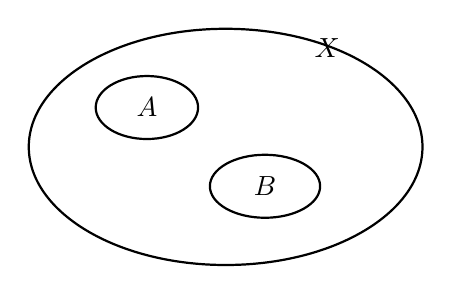
\begin{tikzpicture}[scale=0.5,thick,rotate=-90]
				 \colorlet{MauNet}{black}
				\def\ElipA{(0,0) ellipse  (0.8cm and 1.3cm)}
				\def\ElipB{(2,3) ellipse  (0.8cm and 1.4cm)}
				\def\ElipC{(1,2) ellipse (3cm and 5cm)} 
				\draw[MauNet] \ElipA node[black] {$A$}; 
				\draw[MauNet] \ElipB node[black]  {$B$};
				\draw[MauNet] \ElipC node[black,above  right=1cm] {$X$};
			\end{tikzpicture}
		 }
	\loigiai{ 
		Nhìn biểu đồ, ta thấy $A \cup B  \neq X$.
	} 
\end{ex}

% nguồn: MaHoaNH_TracNghiem_Lop10
\begin{ex}%[0D1H3-2]%[ma:fea28bce]
	Cho $A$, $B$, $C$ là  ba tập hợp được minh họa bằng biểu đồ ven như hình vẽ. Phần gạch sọc trong hình vẽ là tập hợp nào sau đây?
	\choice 
		 {$(A\cup B)\backslash C$}
		{\True $(A\cap B)\backslash C$} 
		{$(A\backslash C)\cup(A\backslash  B)$}
		{$(A\cap B)\cup C$} 
	 \loigiai{
		\begin{center}
			\begin{tikzpicture}[scale=1,font=\footnotesize,line join=round,line cap=round,>=stealth]
					\coordinate  (A) at (0,0);
					\coordinate (B)  at (2,0);
					\coordinate (C) at (1,-1.5); 
					\begin{scope}
						 \clip (A) circle (1.5);
						\fill[pattern=north west lines]  (B) circle (1.5);
					\end{scope}
					 \fill[white] (C) circle (1.5);
					\draw (A) circle  (1.5);
					 \draw (B) circle (1.5);
					\draw (C) circle  (1.5);
					 \path
						 (A)++(90:.6) node[fill=white,above]{$A$}
						(B)++(90:.6)  node[fill=white,above]{$B$}
						(C)++(-90:1)  node[fill=white,above]{$C$};
				\end{tikzpicture}
		\end{center}
		Vì với mỗi phần tử $x$ thuộc phần gạch sọc thì ta thấy $\heva{&x\in A\\&x\in B\\&x\notin  C}$, suy ra $x\in(A\cap B)\backslash C$
	 }
\end{ex}

% nguồn: MaHoaNH_TracNghiem_Lop10
\begin{ex}%[0D1V3-2]%[ma:22c8b9ef]
	Cho hai tập hợp $A=\{0;1\}$ và $B=\{0;1;2;3;4\}$. Số tập hợp $X$ thỏa mãn  $X\subset C_{B}A$ là
	\choice 
		 {$3$}
		{$5$} 
		 {$6$}
		 {\True $8$}
	 \loigiai{
		Ta  có $C_{B}A=B\backslash A=\{2;3;4\}$ có $3$ phần tử nên số tập con $X$ có $2^{3}=8$ (tập).
	 }
\end{ex}

% nguồn: MaHoaNH_TracNghiem_Lop10
\begin{ex}%[0D1V3-2]%[ma:3da70663]
	Cho tập  hợp $A=\{1;2;3;4;5\}$. Tìm số tập hợp $X$ sao cho $A\backslash X=\{1;3;5\}$ và $X\backslash A=\{6;7\}$.
	\choice 
		{\True $1$} 
		 {$2$}
		{$3$} 
		 {$4$}
	 \loigiai{
		Vì $A\backslash X=\{1;3;5\}$ nên $X$ phải chứa  hai phần tử $2$; $4$ và $X$ không chứa các phần tử $1$; $3$$; $ $5$.\\
		Mặt khác $X\backslash A=\{6;7\}$ vậy $X$ phải  chứa $6$; $7$ và các phần tử khác nếu có phải thuộc $A$.\\
		 Vậy $X=\{2;4;6;7\}$.
	} 
\end{ex}

% nguồn: MaHoaNH_TracNghiem_Lop10
\begin{ex}%[0D1K3-2]%[ma:74b73f6b]
	Cho hai tập $A =  \left\{1, 2, 3\right\}$ và $B = \left\{0, 1, 3, 5\right\}$. Tất cả các tập $X$ thỏa mãn $X \subset \left(A \cap B \right)$ là
	\choice 
		{$\varnothing; \left\{1\right\}; \left\{1, 3\right\};  \left\{3\right\}; \left\{1, 3, 5\right\}$}
		 {$\left\{1\right\}; \left\{3\right\}; \left\{1, 3\right\}$}
		{$\varnothing; \left\{1\right\}; \left\{3\right\}$} 
		 {\True $\varnothing; \left\{1\right\}; \left\{3\right\}; \left\{1, 3\right\}$}
	\loigiai{Do $A \cap B = \left\{1, 3\right\}$. Do vậy các tập con $X$ gồm $\varnothing; \left\{1\right\}; \left\{3\right\}; \left\{1, 3\right\}$} 
\end{ex}

% nguồn: MaHoaNH_TracNghiem_Lop10
\begin{ex}%[0D1K3-2]%[ma:61629bf6]
	Cho $A$ và $B$ là hai tập hợp con của tập hợp các số thực $\mathbb{R}$ và thỏa mãn  $A\cap B=\varnothing$. Trong các mệnh đề sau, mệnh đề nào đúng?
	 \choice
		{$C_\mathbb{R}A\subset B$} 
		{$C_\mathbb{R}A=C_\mathbb{R}B$} 
		{\True  $A\subset eq C_\mathbb{R}B$}
		 {$C_\mathbb{R}A\subset C_\mathbb{R}B$}
	\loigiai{Do $A\cap  B=\varnothing$ nên $A\subset eq C_\mathbb{R}B$.}
\end{ex}

% nguồn: MaHoaNH_TracNghiem_Lop10
\begin{ex}%[0D1B3-2]%[ma:79b8f0ec]
	Cho  $A= \lbrace 2;4;6;9 \rbrace$ và $B= \lbrace 1;2;3;4 \rbrace$. Khi đó tập hợp $A \setminus B$ là tập nào sau đây?
	 \choice{$\varnothing $}
		{$ \lbrace 6;9;1;3  \rbrace $}
		{$\lbrace 1;2;3;5  \rbrace $}
		{\True $\lbrace  6;9 \rbrace $}
	\loigiai{$A \setminus B=\{x|\;x\in A \text{ và } x\notin B\}$.\\ Từ giả thiết ta có $A  \setminus B=\lbrace 6;9 \rbrace$.
	 }
\end{ex}

% nguồn: MaHoaNH_TracNghiem_Lop10
\begin{ex}%[0D1B3-2]%[ma:559badcf]
	Cho các tập hợp $A=[m;m+2]$, $B=[-1;2]$.  Điều kiện của $m$ để $A \subset B$ là
	 \choice
		{$\hoac{&m \leq 1 \\& m  \geq 0}$}
		{$\hoac{&m<-1 \\& m>2}$} 
		{\True $-1 \leq  m \leq 0$}
		 {$1 \leq m \leq 2$}
	 \loigiai{
	$A \subset B \Leftrightarrow  \heva{&-1 \leq m \\& m+2 \leq 2}\Leftrightarrow \heva{&m \geq -1 \\& m \leq 0}\Leftrightarrow -1 \leq m \leq 0$.}
\end{ex}

% nguồn: MaHoaNH_TracNghiem_Lop10
\begin{ex}%[0D1B3-2]%[ma:df0da86c]
	Cho $A$ là tập hợp  các hình thoi, $B$ là tập hợp các hình chữ nhật và $C$ là tập hợp các hình vuông. Khi đó
	\choice 
		 {\True $A \cap B=C$}
		{$A  \cup B=C$}
		{$A \setminus B=C$} 
		{$B \setminus A=C$} 
	\loigiai{Ta thấy  hình vuông là hình chữ nhật. Hình vuông cũng là hình thoi. Vậy
	$A  \cap B=C$. }
\end{ex}

% nguồn: MaHoaNH_TracNghiem_Lop10
\begin{ex}%[0D1B3-2]%[ma:ac246cd8]
	Cho  $A=\{x \in \mathbb{R} \mid x^2-4 \ne 0\}$. Tập hợp $A$ viết lại dạng liệt kê là
	 \choice
		 {$\mathbb{R} $}
		 {$\{-2;2\}$}
		{\True  $\mathbb{R} \setminus \{-2;2\}$}
		{$\mathbb{R}  \setminus \{2\}$}
	\loigiai{Ta có $A=\{x \in \mathbb{R} \mid x^2-4 \ne 0\}=\mathbb{R}  \setminus \{-2;2\}$.
	 }
\end{ex}

% nguồn: MaHoaNH_TracNghiem_Lop10
\begin{ex}%[0D1B3-2]%[ma:ea421534]
	Cho  $2$ tập hợp $A=(-7;3),B=(-4;5)$. Chọn khẳng định đúng.
	 \choice
		{\True $A \setminus  B=(-7;-4]$}
		{$A \cap  B=[-4;3)$}
		{$A \cup  B=(-7;-4)$}
		{$A  \setminus B=(-7;-4)$}
	 \loigiai{
	Ta có: $A=(-7;3),B=(-4;5)$  nên $A \setminus B=(-7;-4]$.}
\end{ex}

% nguồn: MaHoaNH_TracNghiem_Lop10
\begin{ex}%[0D1B3-2]%[ma:d7413db3]
	Cho $A=(-\infty;-2]$,  $B=[3;+\infty)$, $C=(0;4)$. Khi đó tập $\left(A\cup B\right)\cap C$ là
	\choice 
		 {$(-\infty;-2]\cup (3;+\infty)$}
		{$(-\infty;-2)\cup [3;+\infty)$} 
		 {\True $[3;4)$}
		{$[3;4]$} 
	\loigiai{ 
	Ta có $A\cup B=(-\infty;-2]\cup [3;+\infty)$. Suy  ra $\left(A\cup B\right)\cap C=[3;4)$.}
\end{ex}

% nguồn: MaHoaNH_TracNghiem_Lop10
\begin{ex}%[0D1B3-2]%[ma:d8155961]
	Chọn kết quả  \bf{sai} trong các kết quả sau
	 \choice
		{$A \cap B=A  \Leftrightarrow A \subset B$}
		 {\True $A \cup B=A \Leftrightarrow A \subset B$}
		{$A \setminus B=A \Leftrightarrow A \cap  B=\varnothing$}
		{$B \setminus A=B\Leftrightarrow  A \cap B=\varnothing$}
	\loigiai{Ta có $A \cup B=A \Leftrightarrow  B \subset A$.
	} 
\end{ex}

% nguồn: MaHoaNH_TracNghiem_Lop10
\begin{ex}%[0D1B3-2]%[ma:040c8e03]
	Cho tập $A=\{0;2;4;6;8\}$; $B=\{3;4;5;6;7\}$. Tập $A\setminus  B$ là
	 \choice
		{$\{0;6;8\}$} 
		 {\True $\{0;2;8\}$}
		{$\{3;6;7\}$} 
		 {$\{0;2\}$}
	 \loigiai{
	Ta có  $A\setminus B=\{0;2;8\}$.}
\end{ex}

% nguồn: MaHoaNH_TracNghiem_Lop10
\begin{ex}%[0D1B3-2]%[ma:b576d053]
	Phần bù của $[-2;1)$ trong $\mathbb{R}$ là 
	 \choice
		{\True $(-\infty;-2) \cup  [1;+\infty)$}
		{$(-\infty;-2)$} 
		 {$(2;+\infty)$}
		 {$(-\infty;1]$}
	\loigiai{ 
	Ta có $\mathbb{R} \setminus [-2;1)=(-\infty;-2) \cup [1;+\infty)$.} 
\end{ex}

% nguồn: MaHoaNH_TracNghiem_Lop10
\begin{ex}%[0D1B3-2]%[ma:501d979e]
	 Cho hai tập hợp $A=\{0;1;2;3;4\}$ và $B=\{2;3;4;5;6\}$. Tập hợp $A \setminus B$ bằng
	 \choice
		 {$\{0\}$}
		{\True $\{0;1\}$} 
		{  $\{1;2\}$}
		{$\{1;5\}$} 
	\loigiai{Ta có  $A \setminus B=\{0;1\}$.
	 }
\end{ex}

% nguồn: MaHoaNH_TracNghiem_Lop10
\begin{ex}%[0D1B3-2]%[ma:5f66d2a9]
	Cho tập hợp  $A=\{1;2;3;5;7\}$, $B=\{2;4;5;6;8\}$. Tập hợp $A \setminus B$ là
	 \choice
		 {$\{4;6;8\}$}
		{\True $\{1;3;7\}$} 
		{$\{1;2;3;4;5;6;7;8\}$} 
		{  $\{2;5\}$}
	\loigiai{Tập  hợp $A \setminus B=\{1;3;7\}$.
	 }
\end{ex}

% nguồn: MaHoaNH_TracNghiem_Lop10
\begin{ex}%[0D1B3-2]%[ma:f58b4006]
	Tập hợp nào sau đây chỉ gồm các số vô  tỷ?
	\choice 
		 {\True $\mathbb{R} \setminus \mathbb{Q}$}
		{$\mathbb{Q} \setminus \mathbb{N}^*$} 
		 {$\mathbb{Q} \setminus \mathbb{Z}$}
		{$\mathbb{R} \setminus  \{0\}$}
	\loigiai{ 
	Ta có $\mathbb{R} \setminus \mathbb{Q}=I$ là tập hợp  các số vô tỷ.}
\end{ex}

% nguồn: MaHoaNH_TracNghiem_Lop10
\begin{ex}%[0D1B3-2]%[ma:86d50357]
	Cho hai tập hợp  $A=\{2;4;6;9\}$ và $B=\{1;2;3;4\}$. Tập hợp $A \setminus B$ bằng tập nào sau đây?
	\choice 
		{$\{1;2;3;5\}$} 
		{$\{1;3;6;9\}$} 
		{\True $\{6;9\}$} 
		 {$\varnothing$}
	\loigiai{Ta có $A \setminus B=\{6;9\}$. 
	 }
\end{ex}

% nguồn: MaHoaNH_TracNghiem_Lop10
\begin{ex}%[0D1B3-2]%[ma:82b78b2b]
	Cho tập $A=\{-2;1;2;3;4\}$, $B=\{x \in  \mathbb{N} \mid x^2-4=0\}$. Mệnh đề nào \bf{sai}?
	\choice 
		{\True  $A \cap B=\{2\}$}
		{$A \cup  B=\{2;-2\}$}
		{$A \setminus B=\{1;3;4\}$} 
		{$A  \cup B=B$}
	\loigiai{Ta có $B=\{x \in \mathbb{N} \mid x^2-4=0\}=\{2\}$, do đó $A  \cap B=\{2\}$.
	} 
\end{ex}

% nguồn: MaHoaNH_TracNghiem_Lop10
\begin{ex}%[0D1B3-2]%[ma:aa4eb10a]
	Tập hợp nào sau  đây chỉ gồm các số vô tỷ?
	\choice 
		{$\mathbb{Q}\setminus \mathbb{N}^*$} 
		{\True $\mathbb{R}\setminus  \mathbb{Q}$}
		{$\mathbb{Q}\setminus  \mathbb{Z}$}
		 {$\mathbb{R}\setminus \{0\}$}
	 \loigiai{
	Tập hợp chỉ  gồm các số vô tỷ là $\mathbb{R}\setminus \mathbb{Q}$.}
\end{ex}

% nguồn: MaHoaNH_TracNghiem_Lop10
\begin{ex}%[0D1K3-2]%[ma:8c6b5165]
	Cho $A=(-\infty;1]$; $B=[1;+\infty)$; $C=(0;1]$. Câu nào sau đây  \textbf{sai}?
	 \choice
		{$\left(A\cup B\right)\setminus C=(-\infty;0]\cup  (1;+\infty)$}
		 {\True $A\cap B\cap C=\{-1\}$}
		{$A\cup  B\cup C=(-\infty;+\infty)$}
		{$\left(A\cap B\right)\setminus C=\varnothing  $}
	\loigiai{ 
	Ta có $A\cap B=\{1\}$ $ \Rightarrow  A\cap B\cap C=\{1\}$.}
\end{ex}

% nguồn: MaHoaNH_TracNghiem_Lop10
\begin{ex}%[0D1K3-2]%[ma:18271721]
	Cho các tập hợp $A=\left\{x\in \mathbb{R}\;|\;x<3\right\}$, $B=\left\{x\in \mathbb{R}\;|\;1<x\leqslant 5\right\}$,\\ $C=\left\{x\in \mathbb{R}\;|\;-2\leqslant x\leqslant 4\right\}$. Khi  đó $\left(B\cup C\right)\setminus \left(A\cap C\right)$ bằng
	 \choice
		 {$[-2;3)$}
		{\True $[3;5]$} 
		 {$(-\infty;1]$}
		 {$[-2;5]$}
	 \loigiai{
		 $A=(-\infty;3)$, $B=(1;5]$, $C=[-2;4]$.\\
	\[\left(B\cup C\right)\setminus \left(A\cap  C\right)=\left\{(1;5]\cup [-2;4]\right\}\setminus \left\{(-\infty;3)\cap [-2;4]\right\}=[-2;5]\setminus [-2;3)=[3;5].\]}
\end{ex}

% nguồn: MaHoaNH_TracNghiem_Lop10
\begin{ex}%[0D1K3-2]%[ma:f4bf06f9]
	Cho hai đa thức $f(x)$ và $g(x)$. Xét các tập hợp $A=\{x\in\mathbb{R}\;\big|\;f(x)=0\}$, $B=\{x\in\mathbb{R}\;\big|\;g(x)=0\}$ và $C=\{x\in\mathbb{R}|f^2(x)+g^2(x)=0\}$. Trong các mệnh đề sau, mệnh đề nào  đúng?
	 \choice
		{$C=A\cup  B$}
		{\True  $C=A\cap B$}
		{$C=A\setminus B$} 
		{$C=B\setminus A$} 
	\loigiai{ 
		Ta có $\forall x\in C\Leftrightarrow f^2(x)+g^2(x)=0\Leftrightarrow \heva{& f(x)=0\\& g(x)=0}\Leftrightarrow\heva{& x\in A\\& x\in B}\Leftrightarrow x\in  A\cap B\Rightarrow C=A\cap B$.
	 }
\end{ex}

% nguồn: MaHoaNH_TracNghiem_Lop10
\begin{ex}%[0D1K3-2]%[ma:ae5e0a7d]
	Cho hai tập hợp $A$ và $B$ có $A\cap B=B$. Có  kết luận gì về tập hợp $B$?
	\choice 
		 {\True $B\subset eq A$}
		{$B\supset A$} 
		 {$C_AB=B$}
		 {$B\cup A=\varnothing$}
	 \loigiai{
		Vì $A\cap B=B\Rightarrow \forall x\in  B\Leftrightarrow x\in A\Rightarrow B\subset eq A$.
	 }
\end{ex}

% nguồn: MaHoaNH_TracNghiem_Lop10
\begin{ex}%[0D1K3-2]%[ma:ffa807be]
	Nếu $P$ là tập hợp hữu hạn phần tử, ta kí hiệu $n(P)$ là số phần tử của tập $P$. Giả sử $A$, $B$ là hai tập có $5$ và $3$ phần tử tương ứng. Trong  các mệnh đề sau, mệnh đề nào đúng?
	 \choice
		{$n\left(A\setminus B\right)=2$} 
		{$n\left(A\cup  B\right)=8$}
		{$n\left(B\setminus A\right)=0$} 
		 {\True $n\left(A\cap B\right)\leq 3$}
	 \loigiai{
		Vì $A$ có  $5$ phần tử và $B$ có $3$ phần tử nên $A\cap B$ là tập có số phần tử không vượt quá $B$ hay $n\left(A\cap B\right)\leq 3$.
	 }
\end{ex}

% nguồn: MaHoaNH_TracNghiem_Lop10
\begin{ex}%[0D1K3-2]%[ma:2520eff2]
	Khẳng định nào sau đây  là đúng?
	\choice 
		 {\True $C_{\mathbb{R}}\mathbb{I}=\mathbb{Q}$}
		{$C_{\mathbb{Q}}\mathbb{Z}=\mathbb{I}$} 
		{$C_{\mathbb{R}}\mathbb{Z}=\mathbb{N}$} 
		{$C_{\mathbb{R}}\mathbb{Q}=\mathbb{Z}$} 
	\loigiai{ 
		 Ta có $C_{\mathbb{R}}\mathbb{I}=\mathbb{Q}$.
	 }
\end{ex}

% nguồn: MaHoaNH_TracNghiem_Lop10
\begin{ex}%[0D1B3-2]%[ma:3f0b27e3]
	Tập hợp $(-2; 4) \backslash[2; 5]$ là tập hợp nào sau  đây?
	\choice 
		{$(-2; 2]$} 
		{\True $(-2; 2)$} 
		{$(-2;  5]$}
		 {$(2; 4)$}
	 \loigiai{
		$(-2;  4) \backslash[2; 5]= (-2; 2)$
	} 
\end{ex}

% nguồn: MaHoaNH_TracNghiem_Lop10
\begin{ex}%[0D1B3-2]%[ma:c0a0f9f1]
	Cho $A$, $B$ là các tập khác rỗng và $A\subset B$. Khẳng định nào sau đây \textbf{sai}? 
	\choice 
		 {$A\cap B=A$}
		 {\True $A\cup B=A$}
		{$B\setminus  A\ne \varnothing$}
		{$A\setminus  B=\varnothing$}
	\loigiai{ 
		Vì $A\subset B$ nên $A\cup B=B$. Vậy mệnh đề  $A\cup B=A$ sai.
	 }
\end{ex}

% nguồn: MaHoaNH_TracNghiem_Lop10
\begin{ex}%[0D1K3-2]%[ma:2824e8a5]
	Cho tập  hợp $A=\left[-1;+\infty\right)$. Tập hợp $C_{\mathbb{R}} A$ là
	 \choice
		 {$\left(-\infty;-1\right]$}
		 {\True $\left(-\infty;-1\right)$}
		{$\mathbb{R}$} 
		{$\varnothing$} 
	 \loigiai{
		Ta có $C_{\mathbb{R}} A= R  \backslash A = (-\infty;-1)$
	} 
\end{ex}

% nguồn: MaHoaNH_TracNghiem_Lop10
\begin{ex}%[0D1B3-2]%[ma:4f275ca5]
	Cho hai tập hợp $A=\left\{ x\in \mathbb{R}\big| x+2\geq 0 \right\}$ và $B=\left\{ x\in \mathbb{R}\big| 5-x\geq 0 \right\}$. Tìm tập hợp  $A \setminus B$.
	\choice 
		{$\left[-2;5  \right]$}
		{$\left[-2;6  \right]$}
		{\True $\left(  5;+\infty \right)$}
		 {$\left( 2;+\infty \right)$}
	\loigiai{ 
		Ta có $A=\left[-2;+\infty\right), B=\left(-\infty;5\right]$.\\ 
		Suy ra $A\setminus  B=\left(5;+\infty \right)$.
	} 
\end{ex}

% nguồn: MaHoaNH_TracNghiem_Lop10
\begin{ex}%[0D1B3-2]%[ma:a6aff2ff]
	Cho $P=(-5;7), Q =(1;+\infty)$. Tập hợp $P \setminus  Q$ là
	 \choice
		 {$[7;+\infty)$}
		 {$(-5;1)$}
		{$(1;7)$} 
		 {\True $(-5;1]$}
	 \loigiai{
		$x \in P \setminus Q \Leftrightarrow \heva{&x \in (-5;7)\\&x \not \in  (1;+\infty)} \Leftrightarrow \heva{&-5 <x<7\\&x \le 1} \Leftrightarrow -5 <x \le 1$.\\
		Do đó $P \setminus Q =(-5;1]$ 
	 }
\end{ex}

% nguồn: MaHoaNH_TracNghiem_Lop10
\begin{ex}%[0D1B3-2]%[ma:9fac841b]
	Cho ba tập hợp $A=\{1; 2; 3; 4; 5; 6; 9\}$, $B=\{0; 2; 4; 6; 8; 9\}$, $C=\{3; 4; 5; 6; 7\}$. Tính tích các phần tử  của tập hợp $A \cap (B \setminus C)$.
	 \choice
		{\True  $18$}
		 {$11$}
		{$2$} 
		{$7$} 
	 \loigiai{
		Ta có  $B\backslash C=\{0; 2; 8; 9\}$. Khi đó $A \cap (B \backslash C)=\{2; 9\}$.\\
		Vậy tích các phần tử là  $2\cdot 9=18$.
	 }
\end{ex}

% nguồn: MaHoaNH_TracNghiem_Lop10
\begin{ex}%[0D1Y3-2]%[ma:8f1f3566]
	Cho dãy số liệu $1; 2; 7; 5; 10; 9; 8$. Số trung vị của  dãy trên bằng bao nhiêu?
	 \choice
		{$ 7  $}
		{\True  $ 6 $}
		{$  8 $}
		{$  2 $ }
	\loigiai{ 
		Xắp xếp mẫu số liệu theo thứ tự  không giảm $1; 2; 5; 7; 8; 9; 10$.\\
		Do  đó trung vị của mẫu số liệu $ M_e=\dfrac{5+7}{2}=6$.
	} 
\end{ex}

% nguồn: MaHoaNH_TracNghiem_Lop10
\begin{ex}%[0D1B3-2]%[ma:b07c36d4]
	Cho hai tập hợp $A =\left\{0,1,2, 3, 4 \right\}$ và $B =\left\{ 2, 3, 4, 5, 6\right\}$. Tìm  tập hợp $(A \setminus B) \cup (B \setminus A)$.
	 \choice
		 {\True $\left\{ 0, 1, 5, 6 \right\}$}
		{$\left\{ 1, 2  \right\}$}
		{$\left\{ 2, 3, 4  \right\}$}
		{$\left\{ 5, 6 \right\}$} 
	\loigiai{ 
		 Ta có $A\setminus B=\left\{ 0, 1\right\}, B\setminus A=\left\{5, 6\right\}$.\\
		Suy ra $(A  \setminus B) \cup (B \setminus A)=\left\{0, 1, 5, 6\right\}$.
	} 
\end{ex}

% nguồn: MaHoaNH_TracNghiem_Lop10
\begin{ex}%[0D1Y3-2]%[ma:4d8eae73]
	Cân nặng $(\mathrm{kg})$ của một  nhóm học sinh lớp 10 cho bởi số liệu sau \linebreak
	 $44; 46; 46; 48; 52; 60; 75; 76; 76; 78$.
	Tìm số  trung vị?
	\choice 
		{$  75 $ }
		{$  52 $}
		{\True  $ 56 $ }
		{$ 60  $}
	\loigiai{ 
		Số trung vị  của mẫu số liệu trên là $ M_e =\dfrac{52+60}{2}=56$.
	} 
\end{ex}

% nguồn: MaHoaNH_TracNghiem_Lop10
\begin{ex}%[0D1K3-2]%[ma:4d1b69cc]
	Cho hai đa thức $f(x)$ và  $g(x)$. Xét các tập hợp
	\begin{center}
		$A=\left\{x\in  \mathbb{R} \mid f(x)=0 \right\}$; $B=\left\{x\in \mathbb{R} \mid g(x)=0 \right\}$; $C=\left\{x\in \mathbb{R} \, \Bigg | \, \dfrac{f(x)}{g(x)} =0 \right\}.$
	\end{center}
	Mệnh  đề nào sau đây là đúng?
	\choice 
		{$C=A\cup B$} 
		{$C=A\cap B$} 
		{\True  $C=A\setminus B$}
		{$C=B\setminus  A$}
	 \loigiai{
		Ta có $\dfrac{f(x)}{g(x)} =0 \Leftrightarrow  \heva{&f(x)=0\\&g(x)\ne 0}$. Do đó $C=A\setminus B$.
	} 
\end{ex}

% nguồn: MaHoaNH_TracNghiem_Lop10
\begin{ex}%[0D1B3-2]%[ma:229bec5c]
	Có bao nhiêu phép toán trên tập hợp? 
	\choice 
		 { $5$}
		{$2$} 
		 {\True $3$}
		{$4$} 
	\loigiai{ Các phép toán trên tập hợp gồm 
		\begin{itemize}
			\item Giao của hai tập hợp; 
			\item Hợp của hai tập  hợp;
			 \item Hiệu và phần bù của hai tập hợp.
		\end{itemize}
	} 
\end{ex}

% nguồn: MaHoaNH_TracNghiem_Lop10
\begin{ex}%[0D1K3-2]%[ma:992cf5ca]
	Trong các mệnh đề sau, mệnh đề nào là mệnh  đề đúng?
	 \choice
		 {$E\subset E\cap F$}
		{$E\cup  F\subset F$}
		{$E\setminus F\subset  F$}
		{\True  $ E=(E\setminus F)\cup (E\cap F)$}
	 \loigiai{
		\begin{itemize}
			\item $E\subset E\cap F$ sai vì chẳng hạn $E=\{1\},F=\{2\}$, khi đó  $E\cap F=\varnothing$.
			\item $E\cup F\subset F$ sai vì chẳng hạn $E=\{1\},F=\{2\}$,  khi đó $E\cup F=\{1;2\}$.
			 \item $E\setminus F\subset F$ sai vì chẳng hạn $E=\{1\},F=\{2\}$, khi đó $E\setminus F=\{1\}$.
		\end{itemize}
	} 
\end{ex}

% nguồn: MaHoaNH_TracNghiem_Lop10
\begin{ex}%[0D1B3-2]%[ma:1e04cd67]
	Cho $A$ là tập tất cả các nghiệm của phương trình $x^2-7x+6=0$, $B$ là tập hợp các số nguyên có giá trị tuyệt đối nhỏ hơn $4$. Hỏi  kết quả nào sau đây là đúng?
	\choice 
		 {$B \setminus A=\varnothing$}
		{$A \cap B=A \cup  B$}
		{\True  $A \setminus B=\{6\}$}
		 {$A \cup B=A$}
	\loigiai{Ta có phương trình $x^2-7x+6=0$ có hai nghiệm $x=1$ và $x=6$, suy ra $A=\{1;6\}$, $B=\{x \in \mathbb{Z} \mid |x|<4  \}=\{-3;-2;-1;0;1;2;3\}$. Khi đó
		\begin{itemize}
			 \item $B \setminus A=\{-3;-2;-1;0;2;3\}$, do đó $B \setminus A \ne \varnothing$;
			\item $A \cap B=\{1\}$, $A \cup B=\{-3;-2;-1;0;1;2;3;6\}$, do đó $A \cap  B \ne A \cup B$;
			\item $A \setminus  B=\{6\}$;
			\item $A \cup  B=\{-3;-2;-1;0;1;2;3;6\} \ne A$.
		\end{itemize}
	} 
\end{ex}

% nguồn: MaHoaNH_TracNghiem_Lop10
\begin{ex}%[0D1B3-2]%[ma:0b19a27d]
	Cho hai tập hợp $ A=\left\lbrace  x\in \mathbb{Z}\,\mid\, x^2+x-6=0 \right\rbrace$, $ B=\left\lbrace x\in \mathbb{N}\,\mid\, 2x^2-3x+1=0 \right\rbrace $. Chọn khẳng định đúng.
	 \choice
		{$  B\setminus A=\left\lbrace 1;2 \right\rbrace $}
		{$ A \cap B=\left\lbrace -3;1;2  \right\rbrace $}
		{\True $ A\setminus B=A  $}
		{$ A  \cup B=\varnothing$}
	\loigiai{ 
	Từ giả thiết ta có 
	\begin{itemize}
		\item $ x^2+x-6=0\Leftrightarrow \hoac{& x=-3\\ &x=2 }$, do $ x \in \mathbb{Z}  \Rightarrow A=\left\lbrace -3;2 \right\rbrace $.
		 \item $ 2x^2-3x+1=0\Leftrightarrow \hoac{& x=1\\ &x=\dfrac{1}{2}}$, do $ x\in \mathbb{N} \Rightarrow B= \left\lbrace 1 \right\rbrace$.
	\end{itemize}
	Vậy $ B\setminus A=\left\lbrace 1 \right\rbrace $, $ A\cap B=\varnothing $, $ A\setminus B=A $, $ A \cup B= \left\lbrace -3;1;2  \right\rbrace $.
	} 
\end{ex}

% nguồn: MaHoaNH_TracNghiem_Lop10
\begin{ex}%[0D1K3-2]%[ma:67bdca4e]
	Cho hai tập hợp $A=\left\{ x\in \mathbb{N} |  x^2<15 \right\}; B=\left\{
	x \in  \mathbb{Z} | -2 \le x \le 2 \right\}$. Tập hợp $A \setminus B$ có bao nhiêu phần tử?
	 \choice
		 {\True $1$}
		{$3$} 
		{$4$} 
		 {$2$}
	\loigiai{ 
		Ta có: $x^2<15 \Leftrightarrow -\sqrt{15} <  x < \sqrt{15}$.\\
		 Mà $x \in \mathbb{N}$ nên $x \in \{0; 1; 2; 3\}$.\\
		$\Rightarrow A=\{0; 1;  2; 3\}$.\\
		Ta có: $\heva{&x\in \mathbb{Z}\\& -2 \le x \le  2} \Leftrightarrow x \in \{-2; -1; 0; 1; 2\}$.\\
		$\Rightarrow B  = \{-2; -1; 0; 1; 2\}$.\\
		Vậy $A \setminus B  = \{3\}$.\\
		$\Rightarrow$ Số phần tử của $A \setminus B$ là  $1$.
	 }
\end{ex}

% nguồn: MaHoaNH_TracNghiem_Lop10
\begin{ex}%[0D1B3-2]%[ma:ce6d7dd3]
	Cho hai tập hợp  $M=\{1;2;3;5\}$ và $N=\{2;6;-1\}$. Xét các khẳng định
	\begin{enumEX}[(I)]{3}
		\item $M\cap  N=\{2\}$
		 \item $N\setminus M=\{1;3;5\}$
		 \item $M\cup N=\{1;2;3;5;6;-1\}.$
	\end{enumEX}
	Có bao nhiêu khẳng  định đúng trong ba khẳng định nêu trên?
	\choice 
		{$0$} 
		{$3$} 
		 {$1$}
		 {\True $2$}
	 \loigiai{
		 Ta có $M\cap N=\{2\}$; $N\setminus M=\{6;-1\}$ và $M\cup N=\{1;2;3;5;6;-1\}$.\\
		Vậy có $2$ khẳng định đúng là (I) và (III). 
	} 
\end{ex}

% nguồn: MaHoaNH_TracNghiem_Lop10
\begin{ex}%[0D1Y3-2]%[ma:048952d9]
	Với $x$ nguyên dương, cho mẫu số liệu sau (đã sắp xếp theo thứ tự) 
	 $$
	\begin{array}{lllllllll}
		4 & 13 & 15 & 4 x-3 & 4 x-1  & 4 x & 22 & 23 & 25
	\end{array}
	 $$
	Tìm $x$, biết rằng số trung vị trong mẫu số liệu trên  bằng $19$.
	\choice 
		 {$x=12$}
		 {$x=14$}
		{\True  $x=5$}
		{$x=15$} 
	\loigiai{ 
		Ta có bảng số liệu trên đã sắp thứ  tự không giảm.\\
		Vì tổng số  liệu của mẫu là $9$ nên trung vị $M_e=4x-1=19\Leftrightarrow x=5$.\\
	} 
\end{ex}

% nguồn: MaHoaNH_TracNghiem_Lop10
\begin{ex}%[0D1B3-2]%[ma:3c5aacdf]
	\immini{Phần tô đậm trong hình vẽ sau biểu  diễn tập hợp nào?\\
	\choice 
		{\True $B\setminus A$} 
		{$A\setminus B$} 
		{$A\cap B$} 
		 {$A\cup B$}}{
		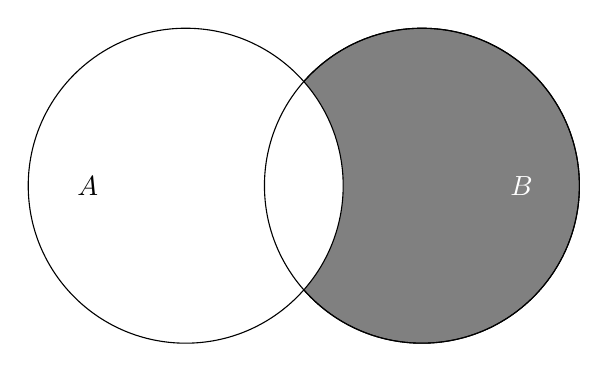
\begin{tikzpicture}[line join=round,line cap=round,>=stealth]
				\tikzset{label style/.style={font=\footnotesize}} 
				 \draw[fill=gray] (3,0) circle (2 cm);
				\draw[fill=white]  (0,0) circle (2 cm);
				 \draw (3,0) circle (2 cm);
				\draw[color=black] (-1.5,0)  node[right] {$A$};
				\draw[color=white]  (4,0) node[right] {$B$};
			\end{tikzpicture}
		} 
	\loigiai{ 
		Phần tô đậm trong hình vẽ  sau biểu diễn tập hợp $B\setminus A$.
	} 
\end{ex}

% nguồn: MaHoaNH_TracNghiem_Lop10
\begin{ex}%[0D1K3-2]%[ma:d999e074]
	\immini{Cho các tập hợp $A$, $B$, $C$. Trong các mệnh đề sau, mệnh  đề nào đúng?
	\choice 
		 {$A\cap\left(B\cup C\right)=A\cup\left(B\cap C\right)$}
		 {$A\cup\left(B\cup C\right)=A\cap\left(B\cap C\right)$}
		{$A\setminus\left(B\cap C\right)=\left(A\setminus B\right)\cap\left(A\setminus  C\right)$}
		{\True $A\setminus\left(B\cup C\right)=\left(A\setminus B\right)\cap\left(A\setminus C\right)$}}{\begin{tikzpicture}[line join=round,line cap=round,>=stealth,thick]
		\tikzset{label  style/.style={font=\footnotesize}}
		\draw[name path=elip1,rotate=35] (0,1) ellipse (2 cm  and 1.5 cm);
		\draw[color=black]  (1,2.2) node[right] {$C$};
		\draw[name path=elip2] (-2,0) ellipse (2  cm and 1.5 cm);
		\draw[color=black] (-4.5,0) node[right]  {$A$};
		\draw[name path=elip1,rotate=-60] (1,-0.5) ellipse (2  cm and 1.5 cm);
		\draw[color=black] (-1.5,-2.5)  node[right] {$B$};
	\end{tikzpicture}
		} 
	\loigiai{ 
		Gọi $x$ là một phần tử thuộc tập hợp $A\setminus\left(B\cup C\right)$, ta có $x \in A; x \not \in B; x  \not \in C$.\\
		Suy ra $x \in A \setminus B$ và $x \in A \setminus C$ hay $x \in \left(A\setminus B\right)\cap\left(A\setminus  C\right)$.\\
		Vậy $A\setminus\left(B\cup C\right)=\left(A\setminus  B\right)\cap\left(A\setminus C\right)$.
	} 
\end{ex}

% nguồn: MaHoaNH_TracNghiem_Lop10
\begin{ex}%[0D1B3-2]%[ma:9b9fe241]
	Cho các tập hợp $A$, $B$, $C$ được minh họa bằng biểu đồ Ven như hình bên. Phần tô màu trong hình là biểu diễn của tập hợp nào sau đây?	\begin{center}
	\def\firstcircle{(0,0) circle (1.5cm)} 
	\def\secondcircle{(45:2cm) circle (1.5cm)} 
	 \def\thirdcircle{(0:2cm) circle (1.5cm)}
	\begin{tikzpicture}
			\draw \firstcircle node[below]  {$A$};
			\draw \secondcircle node [above] {$B$}; 
			 \draw \thirdcircle node [below] {$C$};
			\begin{scope}
				\clip \firstcircle; 
				 \fill[black] \secondcircle;
			\end{scope}
			\begin{scope}
				 \clip \firstcircle;
				 \clip \secondcircle;
				\fill[white]  \thirdcircle;
			\end{scope}
		\end{tikzpicture}
\end{center}
\choice 
	{$A\cap B\cap  C$}
	{$\left(A\setminus C\right)\cup \left(A\setminus B\right)$} 
	 {$\left(A\cup B\right)\setminus C$}
	{\True $\left(A\cap B\right)\setminus  C$}
 \loigiai{
Sử dụng phép toán giao hai tập hợp để tìm $A\cap B$, từ đó suy ra  đáp án $\left(A\cap B\right)\setminus C$.}
\end{ex}


%%%%%%%%%%%%%%%% ĐÚNG/SAI %%%%%%%%%%%%%%%%

% nguồn: MaHoaNH_DungSai_Lop10
\begin{ex}%[0D1N3-2]%[ma:55b2513e]
	Cho các tập hợp $A=\{0;1;2;3;4;5;6\}$, $B=\{-3;-1;1;2;3\}$ và $C=\{x\in  \mathbb{N}|x\text{ là ước của }6\}$.
	\choiceTF 
		{$B\backslash  C=\{-3;-1;1\}$}
		{ $C\backslash  B=\{2;3\}$}
		{\True $C_A  B=\{0;4;5;6\}$}
		{\True $B\backslash A=\{-3;-1\}$} 
	\loigiai{Ta có $A=\{0;1;2;3;4;5;6\}$, $B=\{-3;-1;1;2;3\}$, $C=\{1;2;3;6\}$. 
		\begin{itemchoice}
			\itemch $B\backslash C=\{-3;-1\}$. 
			\itemch $C\backslash B=\{6\}$. 
			\itemch $C_A B=\{0;4;5;6\}$. 
			\itemch $B\backslash  A=\{-3;-1\}$.
		\end{itemchoice}
	 }
\end{ex}

% nguồn: MaHoaNH_DungSai_Lop10
\begin{ex}%[0D1N3-2]%[ma:e3166583]
	Cho các tập hợp $A=\{-2;0;1;3;4\}$, $B=\{0;1;2;5;6\}$ và $C=\{x\in  \mathbb{N}||x|<3\}$.
	\choiceTF 
		{\True $A\backslash B=\{-2;3;4\}$} 
		 { $C\backslash B=\{5;6\}$}
		{ $C_B  C=\varnothing$}
		{ $(A\backslash  C)\cap B=\{-3;-1\}$}
	\loigiai{Ta có  $A=\{-2;0;1;3;4\}$, $B=\{0;1;2;5;6\}$, $C=\{0;1;2\}$.
		\begin{itemchoice}
			 \itemch $A\backslash B=\{-2;3;4\}$.
			 \itemch $C\backslash B=\varnothing$.
			 \itemch $C_B C=\{5;6\}$.
			\itemch  $A\backslash C=\{-2;3;4\}$\\
			$(A\backslash  C)\cap B=\varnothing$.
		\end{itemchoice}
	 }
\end{ex}

% nguồn: MaHoaNH_DungSai_Lop10
\begin{ex}%[0D1H3-2]%[ma:23eaac2a]
	Cho hai tập  hợp: $A=\{-2;-1; 0; 1; 2\}, B=\{-2; 0; 2; 4\}$. Xét tính đúng sai của các khẳng định sau:
	 \choiceTF
		{\True  $A\cap B=\{-2; 0; 2\}$}
		 {$A\cup B=\{-2;-1; 1; 2; 4\}$}
		{\True $A\setminus B=\{-1; 1\}$} 
		 {\True $B\setminus A=\{4\}$}
	 \loigiai{
		\begin{itemchoice}
			\itemch $A\cap  B=\{-2; 0; 2\}$.
			\itemch  $A\cup B=\{-2;-1; 0; 1; 2; 4\}$.
			 \itemch $A\setminus B=\{-1; 1\}$.
			 \itemch $B\setminus A=\{4\}$.
		\end{itemchoice}
	 }
\end{ex}

% nguồn: MaHoaNH_DungSai_Lop10
\begin{ex}%[0D1H3-2]%[ma:82809026]
	Cho đoạn $A=[-5; 1]$ và $B=(-3; 2)$.  Xét tính đúng sai của các khẳng định sau:
	\choiceTF 
		 {$A\cup B=[-3; 2)$}
		{$A\cap B=(-3;  2]$}
		 {\True $A\setminus B=[-5;-3]$}
		 {$C_{\mathbb{R}}(A\cup B)=(-\infty;-5) \cup[1;+\infty)$}
	 \loigiai{
		\begin{itemchoice}
			\itemch $A\cup B=[-5; 2)$. 
			\itemch $A\cap B=(-3; 1]$. 
			 \itemch $A\setminus B=[-5;-3]$.
			\itemch $C_{\mathbb{R}}(A\cup B)=(-\infty;-5)  \cup[2;+\infty)$..
		\end{itemchoice}
	 }
\end{ex}

% nguồn: MaHoaNH_DungSai_Lop10
\begin{ex}%[0D1H3-2]%[ma:1de6353c]
	Cho  hai tập hợp $A=(-1;+\infty), B=(-\infty;-1]$.
	\choiceTF 
		{\True  $A\setminus B=(-1;+\infty)$}
		 {\True $B\setminus A=(-\infty;-1]$}
		{$C_{\mathbb{R}} A=(-\infty;-1)$} 
		 {\True $C_{\mathbb{R}} B=(-1;+\infty)$}
	\loigiai{ 
		\begin{itemchoice}
			\itemch $A\setminus  B=(-1;+\infty)$.
			\itemch $B\setminus A=(-\infty;-1]$. 
			\itemch  $C_{\mathbb{R}} A=(-\infty;-1]$.
			\itemch  $C_{\mathbb{R}} B=(-1;+\infty)$.
		\end{itemchoice}
	 }
\end{ex}

% nguồn: MaHoaNH_DungSai_Lop10
\begin{ex}%[0D1H3-2]%[ma:ea9c1f35]
	Cho hai tập hợp: $A=(-3; 5]$ và $B=(2;+\infty)$.  Xét tính đúng sai của các khẳng định sau:
	 \choiceTF
		 {$A\cap B=(1; 5]$}
		{\True $A\cup  B=(-3;+\infty)$}
		{$A\setminus B=(-2; 2]$} 
		 {\True $C_{\mathbb{R}} A=(-\infty;-3] \cup(5;+\infty)$}
	\loigiai{ 
		\begin{itemchoice}
			\itemch  $A\cap B=(2; 5]$.
			\itemch $A\cup B=(-3;+\infty)$. 
			\itemch  $A\setminus B=(-3; 2]$.
			 \itemch $C_{\mathbb{R}} A=(-\infty;-3] \cup(5;+\infty)$.
		\end{itemchoice}
	 }
\end{ex}

% nguồn: MaHoaNH_DungSai_Lop10
\begin{ex}%[0D1H3-2]%[ma:8033b38f]
	Cho các tập hợp $A=\{0; 1; 2; 3; 4; 5; 6\}, B=\{-3;-1; 1;  2; 3\}$ và $C=\{x \in \mathbb{N} \mid 6~\vdots~ x\}$.
	\choiceTF 
		{$B\setminus C=\{-3;-1; 1\}$} 
		{$C\setminus  B=\{2; 3\}$}
		{\True  $C_A B=\{0; 4; 5; 6\}$}
		{\True $B\setminus A=\{-3;-1\}$} 
	\loigiai{ 
		Ta có  $C=\{1;2;3;6\}$.
		\begin{itemchoice}
			\itemch $B\setminus  C=\{-3;-1\}$.
			 \itemch $C\setminus B=\{6\}$.
			\itemch $C_A  B=\{0; 4; 5; 6\}$.
			\itemch $B\setminus A=\{-3;-1\}$. 
		\end{itemchoice}
	} 
\end{ex}

% nguồn: MaHoaNH_DungSai_Lop10
\begin{ex}%[0D1H3-2]%[ma:316f43d2]
	Cho  hai tập hợp $A=\{x \in \mathbb{R}\mid |x|< 3\}$, $B=[-2; 2]$.
	 \choiceTF
		 {$A\setminus B=\varnothing$}
		{\True  $B\setminus A=\varnothing$}
		{\True $C_{\mathbb{R}} A=(-\infty;-3] \cup[3;+\infty)$} 
		 {$\left(C_{\mathbb{R}} B\right) \cap A=(-\infty;-2) \cup(2;+\infty)$}
	\loigiai{ 
		Ta có $|x|< 3\Leftrightarrow -3<x<3$  suy ra $A=(-3; 3)$.
		\begin{itemchoice}
			 \itemch $A\setminus B=(-3;-2) \cup(2; 3)$.
			\itemch $B\setminus  A=\varnothing$.
			\itemch $C_{\mathbb{R}} A=(-\infty;-3] \cup[3;+\infty)$. 
			 \itemch $\left(C_{\mathbb{R}} B\right) \cap A=(-3;-2) \cup(2; 3)$.
		\end{itemchoice}
	 }
\end{ex}

% nguồn: MaHoaNH_DungSai_Lop10
\begin{ex}%[0D1H3-2]%[ma:3dceba6f]
	Lớp $10C6$  có $18$ học sinh tham gia câu lạc bộ bóng đá và $15$ học sinh tham gia câu lạc bộ bóng rổ. Biết rằng có $10$ học sinh tham gia cả hai câu lạc bộ trên.
	Các khẳng  định sau là đúng hay sai?
	\choiceTF 
		{\True Lớp $10C6$ có $8$ học sinh tham gia câu lạc bộ bóng  đá và không tham gia câu lạc bộ bóng rổ}
		{\True Lớp $10C6$ có $23$ học sinh tham gia ít nhất  một trong hai câu lạc bộ trên}
		{Lớp $10C6$ có $45$ học sinh thì có $25$ học sinh không tham gia câu lạc  bộ bóng đá}
		{Lớp $10C6$ có $45$ học sinh thì có $24$ học sinh không tham gia cả hai  câu lạc bộ}
	\loigiai{ 
		Kí  hiệu:\\
		$A$ là tập hợp học sinh tham gia câu lạc bộ  bóng đá.\\
		$B$ là tập  hợp học sinh tham gia câu lạc bộ bóng rổ.\\
		$E$ là tập  hợp học sinh của lớp.\\
		Ta có thể biểu diễn ba  tập hợp trên bằng biểu đồ Ven như hình sau
		\begin{center}
			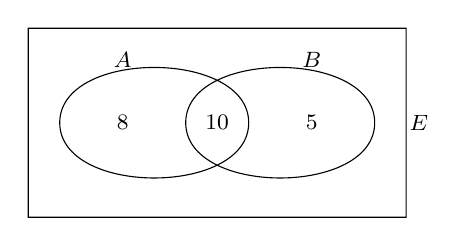
\begin{tikzpicture}[smooth,font=\footnotesize,scale=0.8]
				\def\miena{(0,0) to[bend left=90] (3,0) to[bend left=90] (0,0)}
			\def\mienb{(2,0) to[bend left=90] (5,0) to[bend left=90] (2,0)}
			 \draw \miena \mienb
				(1,0) node{$8$} 
				(4,0)  node{$5$}
				 (2.5,0) node{$10$}
				(1,1) node{$A$} 
				(4,1)  node{$B$}
				(5.7,0)  node{$E$}
				(-0.5,-1.5)--(-0.5,1.5)--(5.5,1.5)--(5.5,-1.5)--cycle; 
			\end{tikzpicture}
		\end{center}
		Khi đó, $A\cap B$ là tập hợp học sinh tham gia cả hai câu lạc bộ trên. Số phần tử của $A$ là $18$, số phần tử của $B$ là $15$, số phần tử của tập  hợp $A\cap B$ là $10$.
		\begin{itemchoice}
			\itemch  Đúng.\\
			Tập hợp các học sinh tham gia câu lạc bộ bóng đá và không tham gia câu lạc bộ bóng rổ là tập hợp $A\setminus B$. Số phần tử của $A\setminus B$ chính là số phần tử của $A$ trừ  đi số phần tử của $A\cap B$. Vậy số học sinh tham gia câu lạc bộ bóng đá và không tham gia câu lạc bộ bóng rổ là $18-10=8$ (học sinh).
			 \itemch Đúng.\\
			Tập hợp các học sinh tham gia ít nhất một trong hai câu lạc bộ trên chính là tập hợp $A\cup B$. Do khi đếm số học sinh tham gia câu lạc bộ bóng đá là $18$, số học sinh tham gia câu lạc bộ bóng rổ là $15$ thì số học sinh tham gia cả hai câu lạc bộ là $10$ được tính hai lần. Vậy số học sinh tham gia ít nhất một trong  hai câu lạc bộ trên là $18+15-10=23$ (học sinh).
			\itemch  Sai.\\
			Số phần tử của $E$ là $45$. Tập hợp các học sinh không tham gia câu lạc bộ bóng đá là phần bù của $A$ trong $E$. Vậy số học sinh không tham gia câu lạc bộ bóng đá là $45-18=27$ (học  sinh).
			\itemch Sai.\\ 
			Tập hợp các học sinh không tham gia cả hai câu lạc bộ là phần bù của $A\cup B$ trong  $E$. Vậy số học sinh không tham gia cả hai câu lạc bộ là $45-23=22$ (học sinh).
	\end{itemchoice}}
\end{ex}

% nguồn: MaHoaNH_DungSai_Lop10
\begin{ex}%[0D1V3-2]%[ma:e2eac782]
	Lớp $10 B_1$ có $7$ học  sinh giỏi Toán, $5$ học sinh giỏi Lý, $6$ học sinh giỏi Hóa, $2$ học sinh chỉ giỏi Toán và Lý, $3$ học sinh chỉ giỏi Toán và Hóa, $1$ học sinh chỉ giỏi cả Lý và Hóa, $1$ học sinh giỏi cả $3$ môn Toán, Lý, Hóa.
	\choiceTF 
		{\True Số  học sinh chỉ giỏi môn Toán là $1$ học sinh}
		{\True Số học sinh chỉ giỏi môn Lý là $1$  học sinh}
		{Số học sinh chỉ giỏi môn Hóa là  $2$ học sinh}
		{\True Số học sinh giỏi  ít nhất một môn (Toán, Lý, Hóa) là $10$ học sinh}
	\loigiai{ 
		Gọi $T$, $L$, $H$ lần lượt là tập hợp các học sinh của lớp giỏi Toán, Lý, Hóa.\\ 
		Theo đề bài ta  có: $|T|=7$; $|L|=5$; $|H|=6$; $|T \cap L|=3$; $|T \cap H|=4$; $|L \cap H|=2$; $|T \cap L \cap H|=3$.
		\begin{itemchoice}
			\itemch Số học sinh chỉ  giỏi môn Toán $7-3-1-2=1$.
			\itemch Số  học sinh chỉ giỏi môn Lý $5-1-1-2=1$.
			\itemch Số  học sinh chỉ giỏi môn Hóa $6-3-1-1=1$.
			 \itemch Số học sinh giỏi ít nhất một môn (Toán, Lý, Hóa) là: $1+2+1+1+1+3+1=10$.
	\end{itemchoice}}
\end{ex}


%%%%%%%%%%%%%%%% TRẢ LỜI NGẮN %%%%%%%%%%%%%%%%

% nguồn: MaHoaNH_TraLoiNgan_Lop10
\begin{bt}%[0D1H3-2]%[ma:5922ad8c]
	Cho hai tập hợp $A=(m-1; 5); B=(3;+\infty), m \in \mathbb{R}$. Có bao  nhiêu số nguyên $m$ để $A\setminus B=\varnothing$.
	 \shortans{2}
	 \loigiai{
		 Điều kiện $m-1< 5\Leftrightarrow m < 6$.\\
		 Để $A\setminus B=\varnothing \Leftrightarrow A\subset B\Leftrightarrow m-1\geq 3\Leftrightarrow m \geq 4$.\\
		Kết hợp điều kiện ban  đầu ta được: $4\leq m < 6$. \\
		 Vậy có $2$ số nguyên thỏa yêu cầu bài toán.
	} 
\end{bt}

% nguồn: MaHoaNH_TraLoiNgan_Lop10
\begin{bt}%[0D1H3-2]%[ma:4da06e69]
	Cho $A$ là tập hợp tất cả các nghiệm của phương trình $x^2-4x+3=0; B$ là tập hợp các số nguyên có giá  trị tuyệt đối nhỏ hơn $4$. Xác định số phần tử của tập hợp $A\setminus B$.
	\shortans{0} 
	 \loigiai{
		Ta có 
		\begin{itemize}
			\item $x^2-7x+6=0\Leftrightarrow\hoac{&x=1\\&x=3} \Rightarrow A=\{1;  3\}$.
			\item $B=\{-3;-2;-1; 0; 1;  2; 3\}$.
		\end{itemize}
		Do đó $A\setminus B=\varnothing$. Suy ra số phần tử của tập hợp $A\setminus B$  là $0$.
	 }
\end{bt}

% nguồn: MaHoaNH_TraLoiNgan_Lop10
\begin{bt}%[0D1H3-2]%[ma:8bd38edd]
	Cho hai tập hợp $X$,  $Y$ thỏa mãn $X\setminus Y=\{7; 15\}$ và $X\cap Y=(-1; 2)$. Xác định số phần tử là số nguyên của $X$.
	 \shortans{4}
	 \loigiai{
		Xét $x$ nguyên  thuộc $X$.
		\begin{itemize}
			\item Nếu $x\in Y$ thì $x\in X\cap Y$. Suy ra $\hoac{&x=0\\&x=1.}  $
			\item Nếu $x\notin Y$ thì  $x\in X\setminus Y $. Suy ra $\hoac{&x=7\\&x=15.} $
		\end{itemize}
		Suy ra $X=\{0;1;7;15\} $. 
		Vậy số phần tử  là số nguyên của $X$ là $4$.
	} 
\end{bt}

% nguồn: MaHoaNH_TraLoiNgan_Lop10
\begin{bt}%[0D1V3-2]%[ma:141a409d]
	Cho hai tập  $A=(-\infty; m)$ và $B=[2m-2; 2m+2]$. Tìm giá trị nguyên của $m$ nhỏ hơn $6$ để $\left(C_{\mathbb{R}} A\right) \cap B\neq \varnothing$.
	 \shortans{6}
	 \loigiai{
		Ta có  $C_{\mathbb{R}} A=[m;+\infty)$.\\
		Để $\left(C_{\mathbb{R}} A\right) \cap B\neq \varnothing \Leftrightarrow 2m+2\geq m \Leftrightarrow m  \geq-2$.\\
		Kết  hợp với $m$ nhỏ hơn $6$ ta có $8$ giá trị thỏa mãn.
	 }
\end{bt}

% nguồn: MaHoaNH_TraLoiNgan_Lop10
\begin{bt}%[0D1V3-2]%[ma:25ed8032]
	Cho $m$ là một tham số thực và hai tập hợp $A=[1-2m; m+3], B=\{x \in \mathbb{R} \mid x \geq 8-5m\}$. Tìm số các giá trị nguyên của  $m$ để $B\setminus A=B$.
	 \shortans{1}
	 \loigiai{
		Ta có $A=[1-2m; m+3]$, $B=[8-5m;+\infty)$.\\ 
		$B\setminus A=B\Leftrightarrow B\cap A=\varnothing \Leftrightarrow\heva{&m+3< 8-5m \\&1-2m \leq m+3} \Leftrightarrow\heva{&6m < 5\\&3m \geq-2} \Leftrightarrow\heva{&m < \dfrac{5}{6} \\&m\geq-\dfrac{2}{3}}\\ \Leftrightarrow-\dfrac{2}{3}  \leq m< \dfrac{5}{6}$.\\
		Vì $m$  nguyên nên $m=0$.
		Vậy có $1$ giá trị nguyên của $m$. 
	} 
\end{bt}

% nguồn: MaHoaNH_TraLoiNgan_Lop10
\begin{bt}%[0D1V3-2]%[ma:3a14fcab]
	Cho tập hợp $X=\{3;-4; 5\}$ có hai tập con $A$ và $B$ (số phần tử của tập $B$ ít hơn số phần tử của tập $A$). Có bao nhiêu cặp  $(A; B)$ mà $\{3;-4\} \cup(A\setminus B)=X$?
	\shortans{11} 
	\loigiai{ 
		Do $\{3;-4\} \cup(A\setminus B)=X$ nên tập hợp $A\setminus B$ phải  chứa phần tử $5$. \\
		Suy ra $5\in  A$, $5\notin B$.\\
		Các tập con của $X$ có phần tử $5$ là $\{5\},\{5;  3\},\{5;-4\},\{5; 3;-4\}$.\\
		Do số phần tử  của tập $B$ ít hơn số phần tử của tập $A$ nên ta có các trường hợp sau\\
		Trường hợp $1$: Nếu $A=\{5\}$ thì $B$ là tập con của $X$ không chứa phần  tử nào, tức là $B=\varnothing$.\\
		Trường hợp $2$: Nếu $A=\{5; 3\}$ thì $B$ là tập con của $X$ chứa ít  hơn hai phần tử và không chứa phần tử $5$, tức là $B=\varnothing, B=\{3\}, B=\{-4\}$.\\
		Trường hợp $3$: Nếu $A=\{5;-4\}$  thì $B$ là tập con của $X$ chứa ít hơn hai phần tử và không chứa phần tử $5$, tức là $B=\varnothing, B=\{3\}, B=\{-4\}$.\\
		Trường hợp $4$: Nếu $A=\{5; 3;-4\}$ thì $B$  là tập con của $X$ chứa ít hơn ba phần tử và không chứa phần tử $5$, tức là $B=\varnothing, B=\{3\}, B=\{-4\}, B=\{3; 4\}$.\\
		Vậy có $1+3+3+4=11$ cặp $(A; B)$  thỏa mãn yêu câu bài toán.
	 }
\end{bt}


%%%%%%%%%%%%%%%% TỰ LUẬN %%%%%%%%%%%%%%%%

% nguồn: MaHoaNH_TuLuan_Lop10
\begin{bt}%[0D1N3-2]%[ma:9cccb8cf]
	Cho hai tập hợp $A=\{1; 2; 3; 7\}$, $B=\{2;  4; 6; 7; 8\}$. Xác định các tập hợp $A \cap B$, $A \cup B$, $A \setminus B$, $B \setminus A$.
	\loigiai{ 
		Ta có $A \cap B=\{2; 7\}$, $A \cup  B=\{1; 2; 3; 4; 6; 7; 8\}$, $A \setminus B=\{1; 3\}$, $B \setminus A=\{4; 6; 8\}$.
	 }
\end{bt}

% nguồn: MaHoaNH_TuLuan_Lop10
\begin{bt}%[0D1H3-2]%[ma:4fc3957f]
	Cho $A$ là tập hợp tất cả  các nghiệm của phương trình $x^2-4x+3=0$; $B$ là tập hợp các số có giá trị tuyệt đối nhỏ hơn $4$. Xác định tập hợp $A \setminus B$.
	\loigiai{ 
		 Ta có $x^2-4x+3=0 \Leftrightarrow \hoac{
		 &x=1 \\
		&x=3} \Rightarrow A=\{1; 3\}$.\\ 
		$B=\{-3;-2;-1;  0; 1; 2; 3\}$. Do đó $A \setminus B=\varnothing$.
	 }
\end{bt}

% nguồn: MaHoaNH_TuLuan_Lop10
\begin{bt}%[0D1V3-2]%[ma:534585cd]
	Lớp 10A có $45$ học sinh trong đó có $25$ em học giỏi môn Toán, $23$ em học giỏi môn Lý, $20$ em học giỏi  môn Hóa, $11$ em học giỏi cả môn Toán và môn Lý, $8$ em học giỏi cả môn Lý và môn Hóa, $9$ em học giỏi cả môn Toán và môn Hóa. Hỏi lớp $10A$ có bao nhiêu bạn học giỏi cả ba môn Toán, Lý, Hóa? (biết rằng mỗi học sinh trong lớp học giỏi ít nhất một trong ba môn Toán, Lý, Hóa).
	 \loigiai{
		Gọi ${T,  L, H}$ lần lượt là tập hợp các học sinh giỏi môn Toán, Lý, Hóa.\\
		Ta  có
		\begin{eqnarray*}
			&|T \cup L \cup  H| &=|T|+|L|+|H|-|T \cap L|-|L \cap H|-|H \cap T|+|T \cap L \cap H|\\
			&45 &=25+23+20-11-8-9+|T \cap L \cap  H|\\
			& \Leftrightarrow|T \cap  L \cap H|& =5.
		\end{eqnarray*}
	Vậy có $5$  học sinh giỏi cả $3$ môn.}
\end{bt}

% nguồn: MaHoaNH_TuLuan_Lop10
\begin{bt}%[0D1K3-2]%[ma:c60c6de2]
	Tìm tất cả các tập $X$ thỏa  mãn $\{1;3\}\cup X= \{0;1;2;3\}$.
	\loigiai{ 
	Ta có $\{0;1;2;3\}\setminus  \{1;3\} = \{0;2\}$ cho nên tất cả các tập $X$ cần tìm là $\{0;2\}$, $\{0;1;2\}$, $\{0;2;3\}$, $\{0;1;2;3\}$.
	 }
\end{bt}

% nguồn: MaHoaNH_TuLuan_Lop10
\begin{bt}%[0D1B3-2]%[ma:d6ca1060]
	Cho $A= \left\{ 1;2;3;4;5 \right\} $, $B=\left\{x \mid  (x^2-2x-3)(x^2-2x-8)=0\right\}$. Tìm $A \cap B$, $A \cup B$, $A \setminus B$.
	 \loigiai{
		Ta có $(x^2-2x-3)(x^2-2x-8)=0 \Leftrightarrow \hoac{& x^2-2x-3=0\\ & x^2-2x-8=0} \Leftrightarrow \hoac{& x=-1\\ & x=3\\ & x=-2\\ & x=4}$. Do  đó $B=\left\{ -2;-1;3;4 \right\} $.\\
		Vậy $A \cap B = \left\{ 3;4 \right\}$,  $A \cup B =\left\{ -2;-1;1;2;3;4;5 \right\}$, $A \setminus B =\left\{ 1;2;5 \right\}$.
	 }
\end{bt}

% nguồn: MaHoaNH_TuLuan_Lop10
\begin{bt}%[0D1B3-2]%[ma:68d512aa]
	Tìm  tập hợp $ A $ và $B$. Biết rằng: $ A \setminus B = \{1,5,7,8\} $; $ A \cap B = \{3,6,9\} $ và $ A \cup B =\{x \in \mathbb{N}|0<x\le 10\} $.
	 \loigiai{
		Ta có $ A  \cup B =\{1,2,3,4,5,6,7,8,9,10\} $.\\
		Vậy  $ A=\{1,3,5,6,7,8,9\} $ và $ B=\{2,3,4,6,9,10\} $.
	} 
\end{bt}

% nguồn: MaHoaNH_TuLuan_Lop10
\begin{bt}%[0D1K3-2]%[ma:8004eb12]
	Cho hai tập hợp $A=\{0;1;3;5\}$ và $B=\{-1;0;2;3\}$. Chứng minh $\left(A\cup  B\right)\setminus \left(A\cap B\right) = \left(A\setminus B\right)\cup \left(B\setminus A\right)$.
	\loigiai{ 
	Ta có $A\cup B=\{-1;0;1;2;3;5\}$ và $A\cap B=\{0;3\}$ nên $\left(A\cup B\right)\setminus \left(A\cap B\right)  = \{-1;1;2;5\}$.\\
	Mặt khác, $A\setminus B=\{1;5\}$ và $B\setminus A=\{-1;2\}$ nên $\left(A\setminus B\right)\cup  \left(B\setminus A\right) = \{-1;1;2;5\}$.\\
	Vậy $\left(A\cup B\right)\setminus \left(A\cap B\right) = \left(A\setminus B\right)\cup \left(B\setminus A\right)$ (điều phải chứng  minh).
	} 
\end{bt}

% nguồn: MaHoaNH_TuLuan_Lop10
\begin{bt}%[0D1K3-2]%[ma:12fa5ecc]
	Cho tập hợp $A=\{1;3;6\}$. Tìm tất cả các tập $X$  thỏa mãn $A\cup X=\{1;2;3;4;5;6\}$ và $A\cap X=\{3\}$.
	 \loigiai{
	 Ta có $\{1;2;3;4;5;6\}\setminus A=\{2;4;5\}$.\\
	Vì  $A\cap X=\{3\}$ nên $3\in X$.\\
	Vậy tất cả  các tập $X$ cần tìm là $\{2;3;4;5\}$, $\{1;2;3;4;5\}$, $\{2;3;4;5;6\}$, $\{1;2;3;4;5;6\}$.
	 }
\end{bt}

% nguồn: MaHoaNH_TuLuan_Lop10
\begin{bt}%[0D1K3-2]%[ma:1423e658]
	Xác định hai tập  hợp $A$ và $B$ biết rằng $A\setminus B=\{1;5;7;8\}$, $B\setminus A=\{2;10\}$ và $A\cap B=\{3;6;9\}$.
	\loigiai{ 
	Vì $A\setminus  B=\{1;5;7;8\}$ nên $\{1;5;7;8\}\subset A$ và $1\notin B$, $5\notin B$, $7\notin B$, $8\notin B$.\hfill$(1)$\\
	Vì $B\setminus A=\{2;10\}$ nên $2\notin A$, $10\notin A$  và $\{2;10\}\subset B$.\hfill$(2)$\\
	Vì $A\cap B=\{3;6;9\}$ nên  $\{3;6;9\}\subset A$ và $\{3;6;9\}\subset B$.\hfill$(3)$\\
	Từ $(1)$, $(2)$ và $(3)$  suy ra $A=\{1;3;5;6;7;8;9\}$, $B=\{2;3;6;9;10\}$.
	 }
\end{bt}

% nguồn: MaHoaNH_TuLuan_Lop10
\begin{bt}%[0D1B3-2]%[ma:156251fd]
	Cho hai tập hợp $A$ và $B$. Tìm các  tập hợp $A\cup B$, $A\cap B$, $A\setminus B$ và $B\setminus A$ với $A=\{-1;2;3;7\}$ và $B=\{x\in\mathbb{R}\mid (x-2)(x-3)=0\}$.
	 \loigiai{
	Ta  có $A=\{-1;2;3;7\}$ và $B=\{2;3\}$. Do đó
	\begin{itemize}
		\item  $A\cup B=\{-1;2;3;7\}$.
		\item $A\cap  B=\{2;3\}$.
		\item $A\setminus B=\{-1;7\}$. 
		 \item $B\setminus A=\varnothing$.
	\end{itemize}
	 }
\end{bt}

% nguồn: MaHoaNH_TuLuan_Lop10
\begin{bt}%[0D1B3-2]%[ma:8bc74714]
	Cho hai tập hợp $A$ và $B$. Tìm các tập hợp  $A\cup B$, $A\cap B$, $A\setminus B$ và $B\setminus A$ với $A=\{x\in\mathbb{N}\mid 3\leq x<7\}$ và $B=\{x\in\mathbb{Z}\mid -1\leq x<5\}$.
	\loigiai{ 
	Ta có  $A=\{3;4;5;6\}$ và $B=\{-1;0;1;2;3;4\}$. Do đó
	\begin{itemize}
		\item $A\cup  B=\{-1;0;1;2;3;4;5;6\}$.
		\item $A\cap  B=\{3;4\}$.
		\item $A\setminus  B=\{5;6\}$.
		 \item $B\setminus A=\{-1;0;1;2\}$.
	\end{itemize}
	 }
\end{bt}

% nguồn: MaHoaNH_TuLuan_Lop10
\begin{bt}%[0D1B3-2]%[ma:db8db0a4]
	Cho  các tập hợp $ A=\{a,b,c,d\} $; $ B=\{b,d,e\} $; $ C=\{a,b,e\} $. Chứng minh các hệ thức
	\begin{enumEX}{2}
		\item $ A \cap (B \setminus C) =(A\cap B)\setminus (A \cap  C) $.
		\item $ A\setminus (B \cap C)=(A \setminus B) \cup  (A\setminus C) $.
	\end{enumEX}
	 \loigiai{
		\begin{enumEX}{2}
			\item Ta  có $ A \cap (B \setminus C)=\{d\}=(A\cap B)\setminus (A \cap C) $.
			\item Ta có $ A\setminus (B  \cap C)=\{a,c,d\}=(A \setminus B) \cup (A\setminus C) $
		\end{enumEX}
	 }
\end{bt}

% nguồn: MaHoaNH_TuLuan_Lop10
\begin{bt}%[0D1K3-2]%[ma:37d548ca]
	Cho hai tập hợp $A=\left\{x\in\mathbb{R}\mid \left(x^3-8\right)\left(2x^2-x-3\right)=0\right\}$ và $B=\left\{x\in\mathbb{Z}\mid 2|x|-5\leq 0\right\}$. Tìm tập hợp $\left(A\cup  B\right)\setminus \left(A\cap B\right)$.
	\loigiai{ 
	 Ta có
	\[\left(x^3-8\right)\left(2x^2-x-3\right)=0 \Leftrightarrow \left[\begin{aligned}&x^3-8=0 \\&2x^2-x-3=0
\end{aligned}\right. \Leftrightarrow \left[\begin{aligned}&x=2 \\&x=-1 \\&x=\dfrac{3}{2}.
\end{aligned}\right.\]
Cho nên $A=\left\{-1;\dfrac{3}{2};2\right\}$.\\ 
Mặt  khác
\[2|x|-5\leq 0 \Leftrightarrow 2|x|\leq 5 \Leftrightarrow |x|\leq \dfrac{5}{2} \Leftrightarrow  -\dfrac{5}{2}\leq x\leq \dfrac{5}{2}.\]
Cho nên $B=\{-2;-1;0;1;2\}$.\\ 
Khi đó $A\cup B= \left\{-2;-1;0;1;\dfrac{3}{2};2\right\}$  và $A\cap B=\{-1;2\}$. Do đó $\left(A\cup B\right)\setminus \left(A\cap B\right) = \left\{-2;0;1;\dfrac{3}{2}\right\}$.
 }
\end{bt}

% nguồn: MaHoaNH_TuLuan_Lop10
\begin{bt}%[0D1B3-2]%[ma:03fadef7]
	Cho  các tập hợp $A=\{1, 2, 3, 7, 8, 12, 13, 15, 24, 29\}$ và $B=\{3, 4, 6, 8, 11, 14, 15, 17, 23, 24\}$.
	\begin{enumerate}
		\item Xác định tập  hợp $A\cup B$ và $A\setminus B$.
		 \item Viết lại tập hợp $A\cap B$ bằng cách chỉ ra tính chất đặc trưng.
	\end{enumerate}
	\loigiai{ 
		\begin{enumerate}
			 \item $A\cup B=\{1,2,3,4,6,7,8,11,12,13,14,15,17,23,24,29\}$.\\
			$A\setminus B=\{1, 2, 7, 12, 13, 29\}$. 
			\item $A\cap B=\{3,8, 15,24\}$.\\ 
			 $A\cap B=\{x\in \mathbb{N}| \,x=n^2-1 \,\text{với} \,n\in \mathbb{N}, 2\le n\le 5\}$.
		\end{enumerate}
	} 
\end{bt}

% nguồn: MaHoaNH_TuLuan_Lop10
\begin{bt}%[0D1B3-2]%[ma:091cd45b]
	Cho $ A=\{x\in\mathbb{R}:2<x\le6\} $, $ B=\{x\in\mathbb{R}:x^2\le9\} $,\\ $  C=\{x\in\mathbb{R}:x\le0 \text{ hay } 3\le x<8\} $.
	\begin{enumerate}
		\item Viết lại các tập hợp $ A $, $ B $, $ C  $ dưới dạng đoạn, khoảng, nữa khoảng.
		\item Tìm $ (A\cup B)\setminus(A\cap B) $, $ \mathrm{C}_\mathbb{R} (A\cup  B\cup C) $
	\end{enumerate}
	 \loigiai{
		\begin{enumerate}
			\item $ A=\left(2;6\right] $, $ B=\left[-3;3\right]  $, $ C=\left(-\infty;0 \right]\cup \left[3;8\right) $.
			\item 
			\begin{itemize}
				\item $  (A\cup B)\setminus(A\cap B)=\left[-3;6\right]\setminus\left(2;3\right]=\left[-3;2\right]\cup \left(3;6\right] $.
				\item Tìm $ \mathrm{C}_\mathbb{R} (A\cup  B\cup C) $.\\
				Ta có  $ (A\cup B\cup C)=\left(-\infty;8\right) $.\\
				Nên suy ra $  \mathrm{C}_\mathbb{R} (A\cup B\cup C)=\left[8;+\infty \right) $.
			\end{itemize}
	\end{enumerate}}
\end{bt}

% nguồn: MaHoaNH_TuLuan_Lop10
\begin{bt}%[0D1B3-2]%[ma:7d460684]
	Cho $ A=\{x \in \mathbb{R} | -1<x\le 5\}  $ và $ B=\{x \in \mathbb{R} | 0 \le x <7\} $. Hãy tìm tập hợp $ C $ thỏa
	\begin{enumEX}{2}
		\item $ C=A \cup  B $.
		\item $ C=A\cap B $. 
		\item $ C= (A\cup  B) \setminus (A \cap B) $.
		\item $ C=(A \setminus B) \cup (B  \setminus A) $.
	\end{enumEX}
	\loigiai{ 
		Ta  có $ A=(-1;5] $ và $ B=[0;7) $, từ đó suy ra
		\begin{enumEX}{2}
			 \item $ C=(-1;7) $.
			\item $  C=[0;5] $.
			\item  $ C=(-1;0) \cup(5;7) $.
			\item $  C=(-1;0) \cup(5;7) $.
		\end{enumEX}
	} 
\end{bt}

% nguồn: MaHoaNH_TuLuan_Lop10
\begin{bt}%[0D1K3-2]%[ma:3ab5fa67]
	Cho  các tập hợp $A$, $B$ và $C$. Chứng minh $A\setminus \left(B\cap C\right)=\left(A \setminus B\right) \cup \left(A\setminus C\right)$.
	 \loigiai{
		Ta phải chứng minh hai  điều
		\begin{itemize}
			 \item $A\setminus\left(B\cap C\right) \subset \left(A \setminus B\right) \cup \left(A\setminus C\right)$.
			Thật vậy,  giả sử
			\begin{eqnarray*}
				x \in A\setminus\left(B\cap C\right) &\Leftrightarrow& \heva{& x \in  A \\ & x \notin B\cap C} \Leftrightarrow \heva{& x \in A\\ & \hoac{& x\notin B\\ & x \notin C}} \\ &\Leftrightarrow & \hoac{& \heva{& x\in A\\ & x\notin B}\\ & \heva{& x\in A\\ & x\notin C}}\Leftrightarrow \hoac{& x\in A\setminus B\\ & x \in A\setminus C}\\&\Leftrightarrow & x \in \left(A \setminus B\right) \cup \left(A\setminus C\right).
			\end{eqnarray*}
			Do đó $A\setminus\left(B\cap C\right) \subset \left(A \setminus B\right) \cup  \left(A\setminus C\right)$ \quad (1).
			\item $\left(A \setminus B\right) \cup \left(A\setminus  C\right) \subset A\setminus \left(B\cap C\right)$.
			Thật vây, giả sử 
			\begin{eqnarray*}
				 x \in \left(A \setminus B\right) \cup \left(A\setminus C\right) &\Leftrightarrow& \hoac{& x \in \left(A \setminus B\right)\\ & x\in \left(A\setminus C\right) }\Leftrightarrow \hoac{& \heva{& x \in A\\ & x\notin B}\\ & \heva{& x\in A\\ & x\notin C}}\\&\Leftrightarrow & \heva{& x\in A\\ & \hoac{& x\notin B\\ & x \notin C}}\Leftrightarrow \heva{& x\in A\\ & x\notin B\cap C}\\
				&\Leftrightarrow  & x\in A\setminus \left(B\cap C\right).
			\end{eqnarray*}
			Vậy $\left(A \setminus B\right)  \cup \left(A\setminus C\right) \subset A\setminus \left(B\cap C\right)$ \quad (2).
		\end{itemize}
		Từ (1) và (2) ta có điều  phải chứng minh.
	} 
\end{bt}

% nguồn: MaHoaNH_TuLuan_Lop10
\begin{bt}%[0D1B3-2]%[ma:38c121b0]
	Cho các tập hợp $A=(-3;6]$,  $B=(4;+\infty)$. Tìm $A\cup B$, $A\cap B$, $\mathrm{C}_{\mathbb{R}}A$.
	 \loigiai{
		\begin{center}
			 Tập $A$\\
			\begin{tikzpicture}[x=.5cm,scale=1,font=\footnotesize,line join=round,line cap=round,>=stealth]
					\fill[pattern=north east  lines](-5,-0.15) rectangle (-3,0.15);
					\fill[pattern=north east  lines](-5,-0.15) rectangle (-3,0.15);
					\fill[pattern=north east lines](6,-0.15)  rectangle (8,0.15);
					\draw[->]  (-5,0)--(8,0);
					\draw  (-3,0) node {$\big ($}
						(-3,0) node[below=6pt]{$-3$}; 
					\draw (6,0)  node {$\big]$}
						(6,0) node[below=6pt]{$6$}; 
				\end{tikzpicture}
		\end{center}
		\begin{center}
			Tập $B$\\ 
			\begin{tikzpicture}[x=.5cm,scale=1,font=\footnotesize,line join=round,line cap=round,>=stealth]
					\fill[pattern=north west lines](-5,-0.15) rectangle  (4,0.15);
					\draw[->]  (-5,0)--(8,0);
					\draw (4,0) node {$\big  ($}
						(4,0)  node[below=6pt]{$4$};
				\end{tikzpicture}
		\end{center}
		\begin{center}
			Tập $A\cup B=(-3;+\infty)$\\ 
			\begin{tikzpicture}[x=.5cm,scale=1,font=\footnotesize,line join=round,line cap=round,>=stealth]
					\fill[pattern=north east  lines](-5,-0.15) rectangle (-3,0.15);
					\draw[->] (-5,0)--(8,0); 
					 \draw (-3,0) node {$\big ($}
						(-3,0) node[below=6pt]{$-3$}; 
				\end{tikzpicture}
		\end{center}
		\begin{center}
			Tập $A\cap  B=(4;6]$\\
			\begin{tikzpicture}[x=.5cm,scale=1,font=\footnotesize,line join=round,line cap=round,>=stealth]
					 \fill[pattern=north east lines](-5,-0.15) rectangle (4,0.15);
					\fill[pattern=north east lines](6,-0.15) rectangle (8,0.15); 
					\draw[->] (-5,0)--(8,0); 
					\draw (4,0) node  {$\big ($}
						(4,0)  node[below=6pt]{$4$};
					\draw (6,0) node {$\big]$} 
						(6,0) node[below=6pt]{$6$}; 
				\end{tikzpicture}
		\end{center}
		\begin{center}
			Tập $\mathrm{C}_{\mathbb{R}}A=\mathbb{R}\setminus A=(-\infty;-3] \cup  (6;+\infty)$\\
			\begin{tikzpicture}[x=.5cm,scale=1,font=\footnotesize,line join=round,line cap=round,>=stealth]
					\fill[pattern=north east lines](-3,-0.15) rectangle (6,0.15); 
					\draw[->] (-5,0)--(8,0); 
					\draw (-3,0)  node {$\big]$}
						(-3,0) node[below=6pt]{$-3$}; 
					\draw (6,0) node  {$\big ($}
						(6,0) node[below=6pt]{$6$}; 
				\end{tikzpicture}
		\end{center}
	 }
\end{bt}

% nguồn: MaHoaNH_TuLuan_Lop10
\begin{bt}%[0D1K3-2]%[ma:6633bc18]
	Chứng minh rằng: 
	\begin{listEX}[2]
		 \item $ A \subset A \cup B$;
		 \item $ B \subset A \cup B$;
		\item $A \cup B  = B \cup A$;
		\item $(A \cup B) \cup C  = A \cup (B \cup C)$;
		\item $A  \cup B = B \Leftrightarrow A \subset B$;
		\item $A \cap B  = B \cap A$;
		\item $(A \cap B) \cap C = A \cap (B \cap C)$; 
		\item $A \cap B = B  \Leftrightarrow B \subset A$;
		\item $A \cap B  \subset B$;
		\item $A \cap B \subset A$; 
		\item $A \setminus B \subset  A$;
		\item $B \setminus A \subset B$; 
		\item  $A \cap B \subset A \cup B$;
		\item $A \cup (B \cap C) = (A \cup  B) \cap (A \cup C)$;
		\item $A \cap (B \cup C) = (A \cap B) \cup  (A \cap C)$;
		\item $A  \setminus B = A \setminus (A \cap B)$;
		\item $A \setminus B = \varnothing \Leftrightarrow A \subset B$; 
		\item Nếu $A \subset B$ thì $A \cap B =  A$.
	\end{listEX}
	\loigiai{ 
		\begin{enumEX}{1}
			\item $a\in A \Rightarrow \hoac{&a\in A\\&a\in B} \Rightarrow a\in A\cup B \Rightarrow A \subset A  \cup B$.
			\item $b\in B\Rightarrow b\in B \Rightarrow \hoac{&b\in A\\&b\in B} \Rightarrow b\in A\cup B \Rightarrow B \subset  A\cup B$.
			\item $a \in A \cup B \Leftrightarrow \hoac{& a \in A \\ &a \in B} \Leftrightarrow \hoac{& a \in B \\ &a \in A} \Leftrightarrow a \in B \cup A.$\\ 
			Vậy  $A\cup B = A \cup B$.
			\item Lấy $a \in (A \cup B) \cup C \Leftrightarrow \hoac{& a \in A \cup B \\ &a \in C} \Leftrightarrow \hoac{& a \in A \\ &a \in B \\ & a \in C} \Leftrightarrow \hoac{& a  \in A \\ &a \in B \cup C} \Leftrightarrow a \in A \cup (B \cup C).$\\
			Vậy $(A \cup B) \cup C = A  \cup (B \cup C)$.
			\item Chứng minh $A \cup B = B \Leftrightarrow A \subset  B$.
			\begin{enumerate}
				\item[Thuận:] $A \cup B = B \Rightarrow A \subset B$.\\ Lấy $a \in A \Rightarrow \hoac{& a \in A \\ &a \in B} \Rightarrow a \in A \cup B \Rightarrow a \in B$ (do $A \cup  B = B$) $\Rightarrow a \in A \subset B$. Vậy $A \cup B = B \Rightarrow A \subset B$.
				\item[Đảo:] $ A  \subset B \Rightarrow A \cup B = B $. \\
				Lấy $a \in A \cup B \Leftrightarrow \hoac{& a \in A \\ &a \in B} \Leftrightarrow \hoac{& a \in B \\ &a \in B}$ (do $A \subset B$) $\Leftrightarrow a \in B \Rightarrow A \cup B = B$. Vậy $ A \subset  B \Rightarrow A \cup B = B $. \\
				Vậy $A \cup B = B  \Leftrightarrow A \subset B$.
			\end{enumerate}
			\item $a \in A \cap B \Leftrightarrow \heva{& a \in A \\  &a \in B} \Leftrightarrow \heva{& a \in B \\ &a \in A} \Leftrightarrow a \in B \cap A.$\\
			Vậy  $A \cap B = B \cap A$.
			\item Lấy $a \in (A \cap B) \cap C \Leftrightarrow \heva{& a \in A \cap B \\ &a \in C} \Leftrightarrow \heva{& a \in A  \\ &a \in B \\ & a \in C} \Leftrightarrow \heva{& a \in A \\ &a \in B \cap C} \Leftrightarrow a \in A \cap (B \cap C).$\\
			Vậy $(A \cap B) \cap  C = A \cap (B \cap C)$.
			\item Chứng minh $A \cap B = B \Leftrightarrow B  \subset A$.
			\begin{enumerate}
				\item[Thuận:] $A \cap B = B  \Rightarrow B \subset A$.\\ Lấy $a \in B \Rightarrow a \in A \cap B \; (\text{do } A \cap B = B) \Rightarrow \heva{& a \in A \\ &a \in B} \Rightarrow a \in A$ Vậy $A \cap B = B \Rightarrow B \subset A$.
				\item[Đảo:] $ B \subset A \Rightarrow A \cap B =  B$. \\
				Lấy $a \in A \cap B \Leftrightarrow  \heva{& a \in A \\ & a \in B} \Leftrightarrow a \in B$ (do $A \subset B$) $ \Rightarrow A \cap B = B$. Vậy $ B \subset A \Rightarrow A \cap B = B$. \\
				Vậy $A \cap B = B \Leftrightarrow B \subset  A$.
			\end{enumerate}
			\item $a  \in A \cap B \Rightarrow \heva{& a \in A \\ &a \in B} \Rightarrow a \in B $. \\Vậy $A \cap B \subset B$.
			\item $a \in A \cap B \Rightarrow \heva{& a \in A \\ &a \in B} \Rightarrow  a \in A $. \\Vậy $A \cap B \subset A$.
			\item $a \in A \setminus B \Rightarrow \heva{&  a \in A \\ &a \not \in B} \Rightarrow a \in A \Rightarrow A \setminus B \subset A$.
			\item $a \in B \setminus A \Rightarrow \heva{& a \in B \\ &a \not \in A} \Rightarrow a \in B \Rightarrow B \setminus  A \subset B$.
			\item $a\in A\cap B \Rightarrow \heva{&a\in A\\& a\in B} \Rightarrow a\in A \Rightarrow \hoac{&a\in A\\& a\in B} \Rightarrow a\in  A \cup B$.\\
			 Vậy $A\cap B \subset A\cup B$.
			\item $a \in  A \cup (B \cap C) \Leftrightarrow \hoac{&a\in A\\& a\in B\cap C} \Leftrightarrow \hoac{&a\in A\\&\heva{&a\in B\\&a\in C}} \Leftrightarrow \heva{&\hoac{&a\in A\\&a\in B}\\&\hoac{&a\in A\\&a\in C}} \Leftrightarrow a\in (A \cup B) \cap (A \cup C)$.\\
			Vậy $A \cup (B \cap C) = (A \cup  B) \cap (A \cup C)$.
			\item $a\in A \cap (B \cup C) \Leftrightarrow \heva{&a\in A\\&a\in B\cup C} \Leftrightarrow \heva{&a\in A\\&\hoac{&a\in B\\&a\in C}}\Leftrightarrow \hoac{&\heva{&a\in A\\& a\in B}\\&\heva{&a\in A\\&a\in C}} \Leftrightarrow a \in (A  \cap B) \cup (A \cap C)$.\\
			Vậy $A \cap (B \cup C) = (A \cap B) \cup  (A \cap C)$.
			\item $a\in A \setminus B \Leftrightarrow \heva{&a\in A\\& a\notin B}\Leftrightarrow \heva{&a\in A\\& a\notin A\cap  B} \Leftrightarrow a\in A \setminus (A \cap B)$.\\
			Vậy $A \setminus B = A \setminus (A \cap B)$. 
			\item Để chứng  minh $A\setminus B=\varnothing \Leftrightarrow A\subset B$ ta chứng minh mệnh đề phản đảo của nó là $A\setminus B\neq\varnothing \Leftrightarrow A\not\subset B$.\\
			\begin{enumerate}
				\item[Thuận:] $A\setminus B\neq \varnothing\Rightarrow \exists  x\in A\setminus B\Rightarrow \heva{x\in A\\ x\not\in B}\Rightarrow A\not\subset B$.
				\item[Đảo:] $A\not \subset B\Rightarrow \exists x \text{ sao cho  } \heva{x\in A\\ x\not \in B}\Rightarrow x\in A\setminus B\Rightarrow A\setminus B\neq \varnothing$.
			\end{enumerate}
			\item $a\in A \cap B \Leftrightarrow \heva{&a\in A\\& a\in B \; (\text{luôn đúng vì} \; A\subset B}  \Leftrightarrow a\in A$.\\
			Vậy nếu $A \subset B$ thì $A \cap B  = A$.
	\end{enumEX}}
\end{bt}
